\documentclass[preprint]{aastex}  % USE THIS TO MAKE BIB, THEN FORMAT USING EMULATEAPJ
%\documentclass[twocolumn,numberedappendix]{emulateapj}
\shorttitle{Transit Dish for 21cm Intensity Mapping}
\shortauthors{XXX Authors}

\usepackage{amsmath, amsthm, amssymb}
\usepackage{graphicx}
\usepackage[figuresright]{rotating}
%\usepackage{rotating}
\usepackage{natbib}
\usepackage{morefloats}
%\usepackage{pdflscape}
%\usepackage{lscape}
\citestyle{aa}

\newcommand{\BigO}[1]{\mathcal{O}(#1)}
\def\k{\mathbf{k}}
\def\r{\mathbf{r}}
\def\V{\mathbb{V}}
\def\At{\tilde{A}}
\def\Vt{\tilde{V}}
\def\Tt{\tilde{T}}
\def\tb{\langle T_b\rangle}

\begin{document}
\title{A Transit Dish Design for High-Redshift 21cm Intensity Mapping Experiments}

\author{
%Aaron R. Parsons\altaffilmark{1,2},
%Adrian Liu\altaffilmark{1},
%James E. Aguirre\altaffilmark{3},
%Zaki S. Ali\altaffilmark{1},
%Richard F. Bradley\altaffilmark{4,5,6},
%Chris L.  Carilli\altaffilmark{7},
%David R. DeBoer\altaffilmark{2},
%Daniel C. Jacobs\altaffilmark{8},
%David F. Moore\altaffilmark{3},
%Jonathan C. Pober\altaffilmark{1},
}

%\altaffiltext{1}{Astronomy Dept., U. California, Berkeley, CA}
%\altaffiltext{2}{Radio Astronomy Lab., U. California, Berkeley, CA}
%\altaffiltext{3}{Dept. of Physics and Astronomy, U. Pennsylvania, Philadelphia, PA}
%\altaffiltext{4}{Dept. of Electrical and Computer Engineering, U. Virginia, Charlottesville, VA}
%\altaffiltext{5}{National Radio Astronomy Obs., Charlottesville, VA}
%\altaffiltext{6}{Dept. of Astronomy, U. Virginia, Charlottesville, VA}
%\altaffiltext{7}{National Radio Astronomy Obs., Socorro, NM}
%\altaffiltext{8}{School of Earth and Space Exploration, Arizona State U., Tempe, AZ}
%\altaffiltext{9}{Square Kilometer Array, South Africa Project, Cape Town, South Africa}
%\altaffiltext{10}{Cavendish Lab., Cambridge, UK}

\begin{abstract}
\end{abstract}

\section{Introduction}

\begin{itemize}
\item importance of frequency smoothness
\item collecting area
\end{itemize}

\section{Background}
\label{sec:background}

\begin{itemize}
\item $\tau$-modes, wedge, EoR window
\item geometric interpretation of $\tau$-modes
\end{itemize}

\section{Geometric Constraints}
\label{sec:geometry}

\begin{itemize}
\item first principles of EoR window, how that maps to a specification for design
\item cost analysis
\item critically constrained design
\item symmetric on-axis parabaloid, for reasons of symmetry in polarization response
\end{itemize}

\section{Design and Construction}
\label{sec:design}

\subsection{bent pipes as approximation to parabola}
The construction method is based on the use of a reasonably stiff spar supported at a few points as a low-pass spatial filter.  Additionally, a moment-loaded beam naturally attains a parabolic shape, depending on the loading, the moment of intertia and the material's Young's modulus (see {\em e.g.} http://ruina.tam.cornell.edu/ Courses/~ME4730/ Rand4770 Vibrations/ BeamFormulas.pdf).  In this instance we fix the angle at the rim ($r_e$) of 7m and at a hub radius ($r_h$) of about 45 cm, so between those two points, the effective angle is $(r_e-r_h)/(2F)$, where $F$ is the focal length (4.5m).  Equating that angle to the angle of the cantilevered beam (using scenario 5 of the web-site) we find
\begin{equation}
y = \left(\frac{r_e-r_h}{L}\right)\frac{x^2}{4F}
\end{equation}
where $L$ is the length of the beam.
Assuming, $(r_e-r_h) \approx L$ (in this case, the ratio is 0.91) we find we have the equation for our desired parabola.  Note that we do not contend that this figure over the entire length of the actual beam achieves this, but merely that if properly held and loaded it tends to the right shape.

In our construction, we hold the spar at three locations at the proper location and angle and then rely on the fairly stiff spar to "filter" out any higher frequency ripples and on the physics to give us the overall general shape.

\begin{figure}[H]
	\begin{center}
	
\includegraphics[width =\textwidth]{empty}
	\caption{THIS FIGURE SHOWS THE ANALYSIS ON PARABOLA
\label{Fig:} }
	\end{center}
\end{figure}

\begin{figure}[H]
	\begin{center}
	
\includegraphics[width =\textwidth]{empty}
	\caption{THIS FIGURE SHOWS THE PHOTGRAMMRY ANALYSIS 
\label{Fig:} }
	\end{center}
\end{figure}

\subsection{faceting}
The construction of the surface stretches mesh panels over adjacent spars, so the surface is not a true paraboloid but rather a faceted parabola, although note that the construction does pull down the mesh mid-panel to both better approximate a paraboloid as well as to hold the mesh.

If we assume an actual faceted parabola ({\em i.e.} the mesh if perfectly flat between adjacent spars) we can calculate the rms deviation from a paraboloid for various spar configurations.  For this antenna, we chose 12 spars out to 1.45m, then transitioning to 24 spars.  Choosing just 12 spars all the way out to the rim yields an rms of 6.9cm (corresponding to a Ruze loss of almost 18\% at 150 MHz), as opposed to 1.7cm (for about 1 \% loss).

\begin{figure}[H]
	\begin{center}
	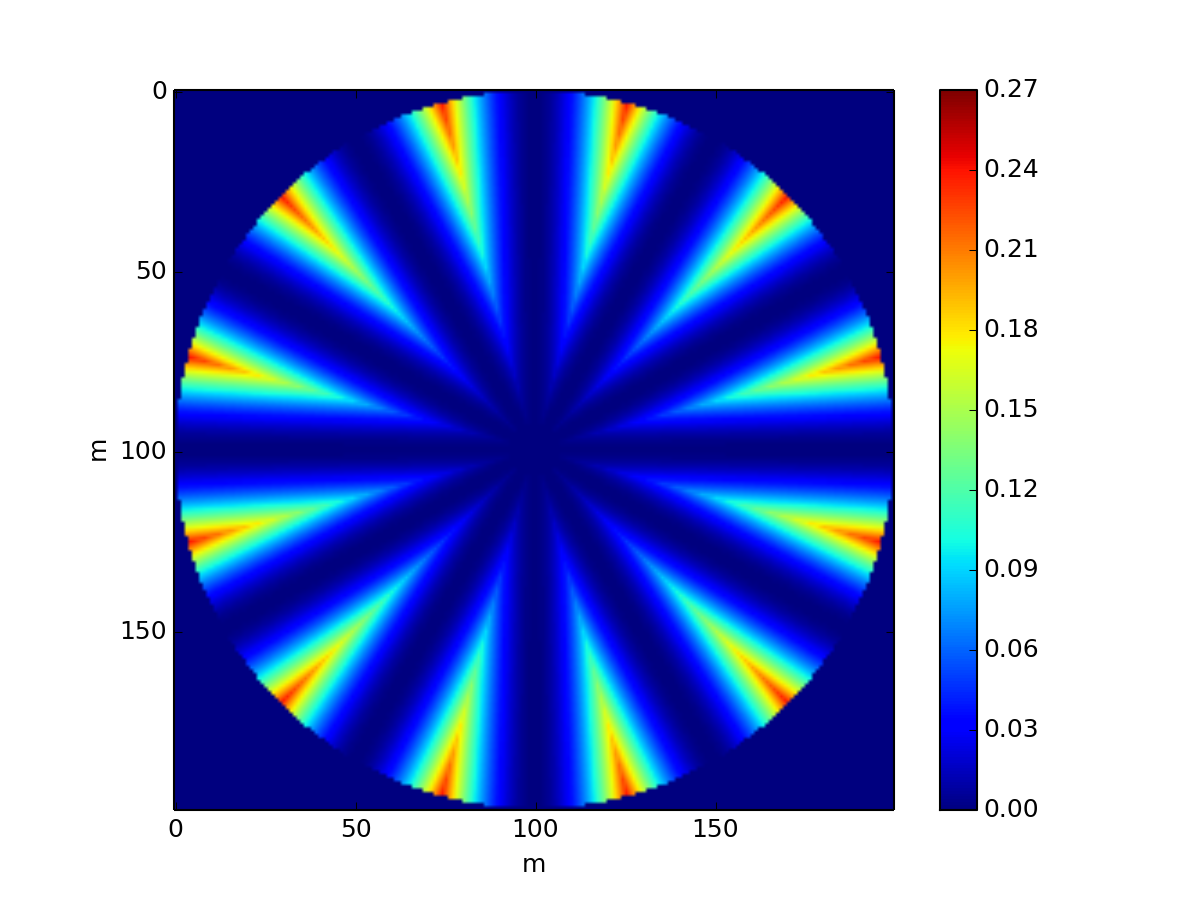
\includegraphics[width =0.45\textwidth]{dish_plots/12spar.png}
	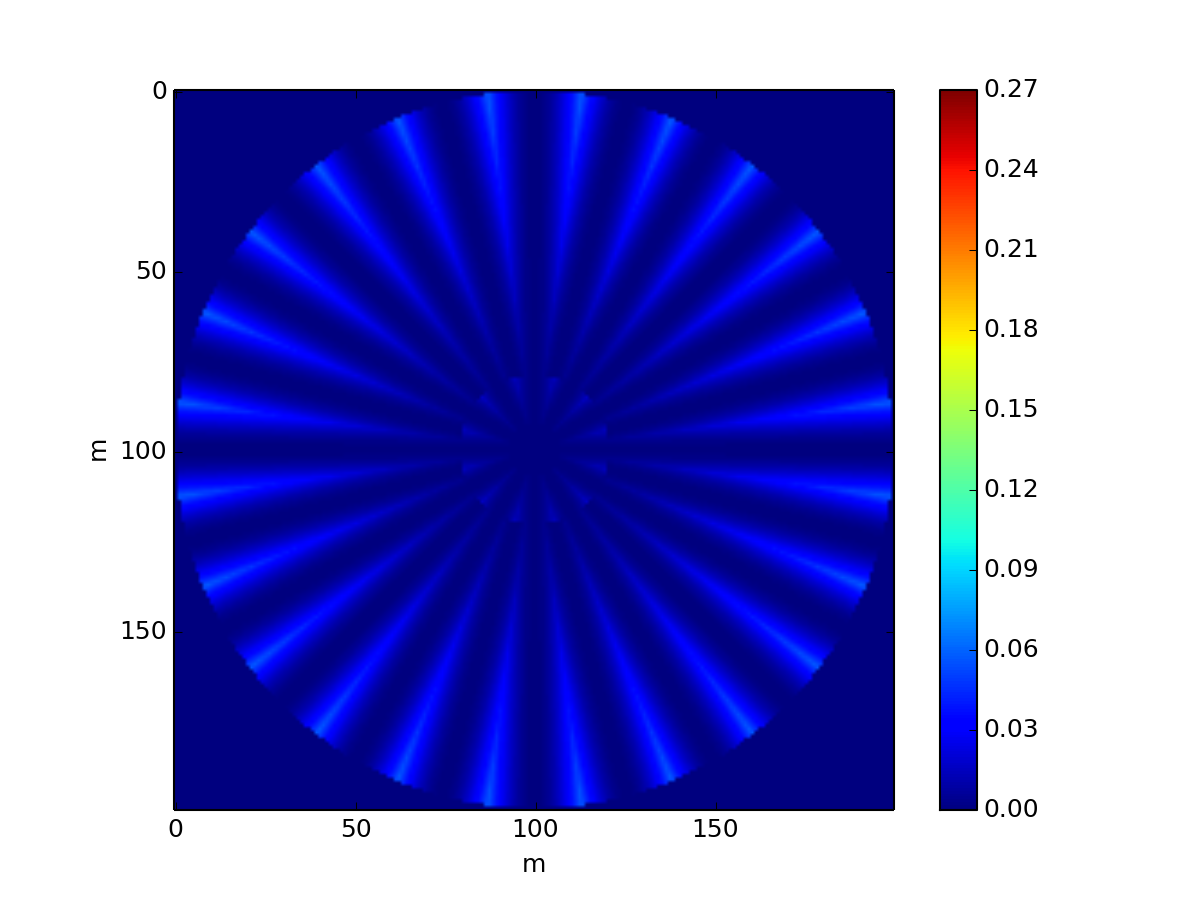
\includegraphics[width = 0.45\textwidth]{dish_plots/special_spar.png}
	\caption{Contour plots of the facet deviations from a paraboloid for 12 spars (left) and the 12-to-24 spar design (right).
\label{Fig:facets} }
	\end{center}
\end{figure}

\subsection{shielding}
The panels across the dish surface are made out of 6 different dimensions of galvanized wire cloth $\frac{1}{4}$"; employing different dimensions at different heights to reduce the surface bumps produced during installation.

\subsection{splash cone}
\begin{figure}[H]
	\begin{center}
	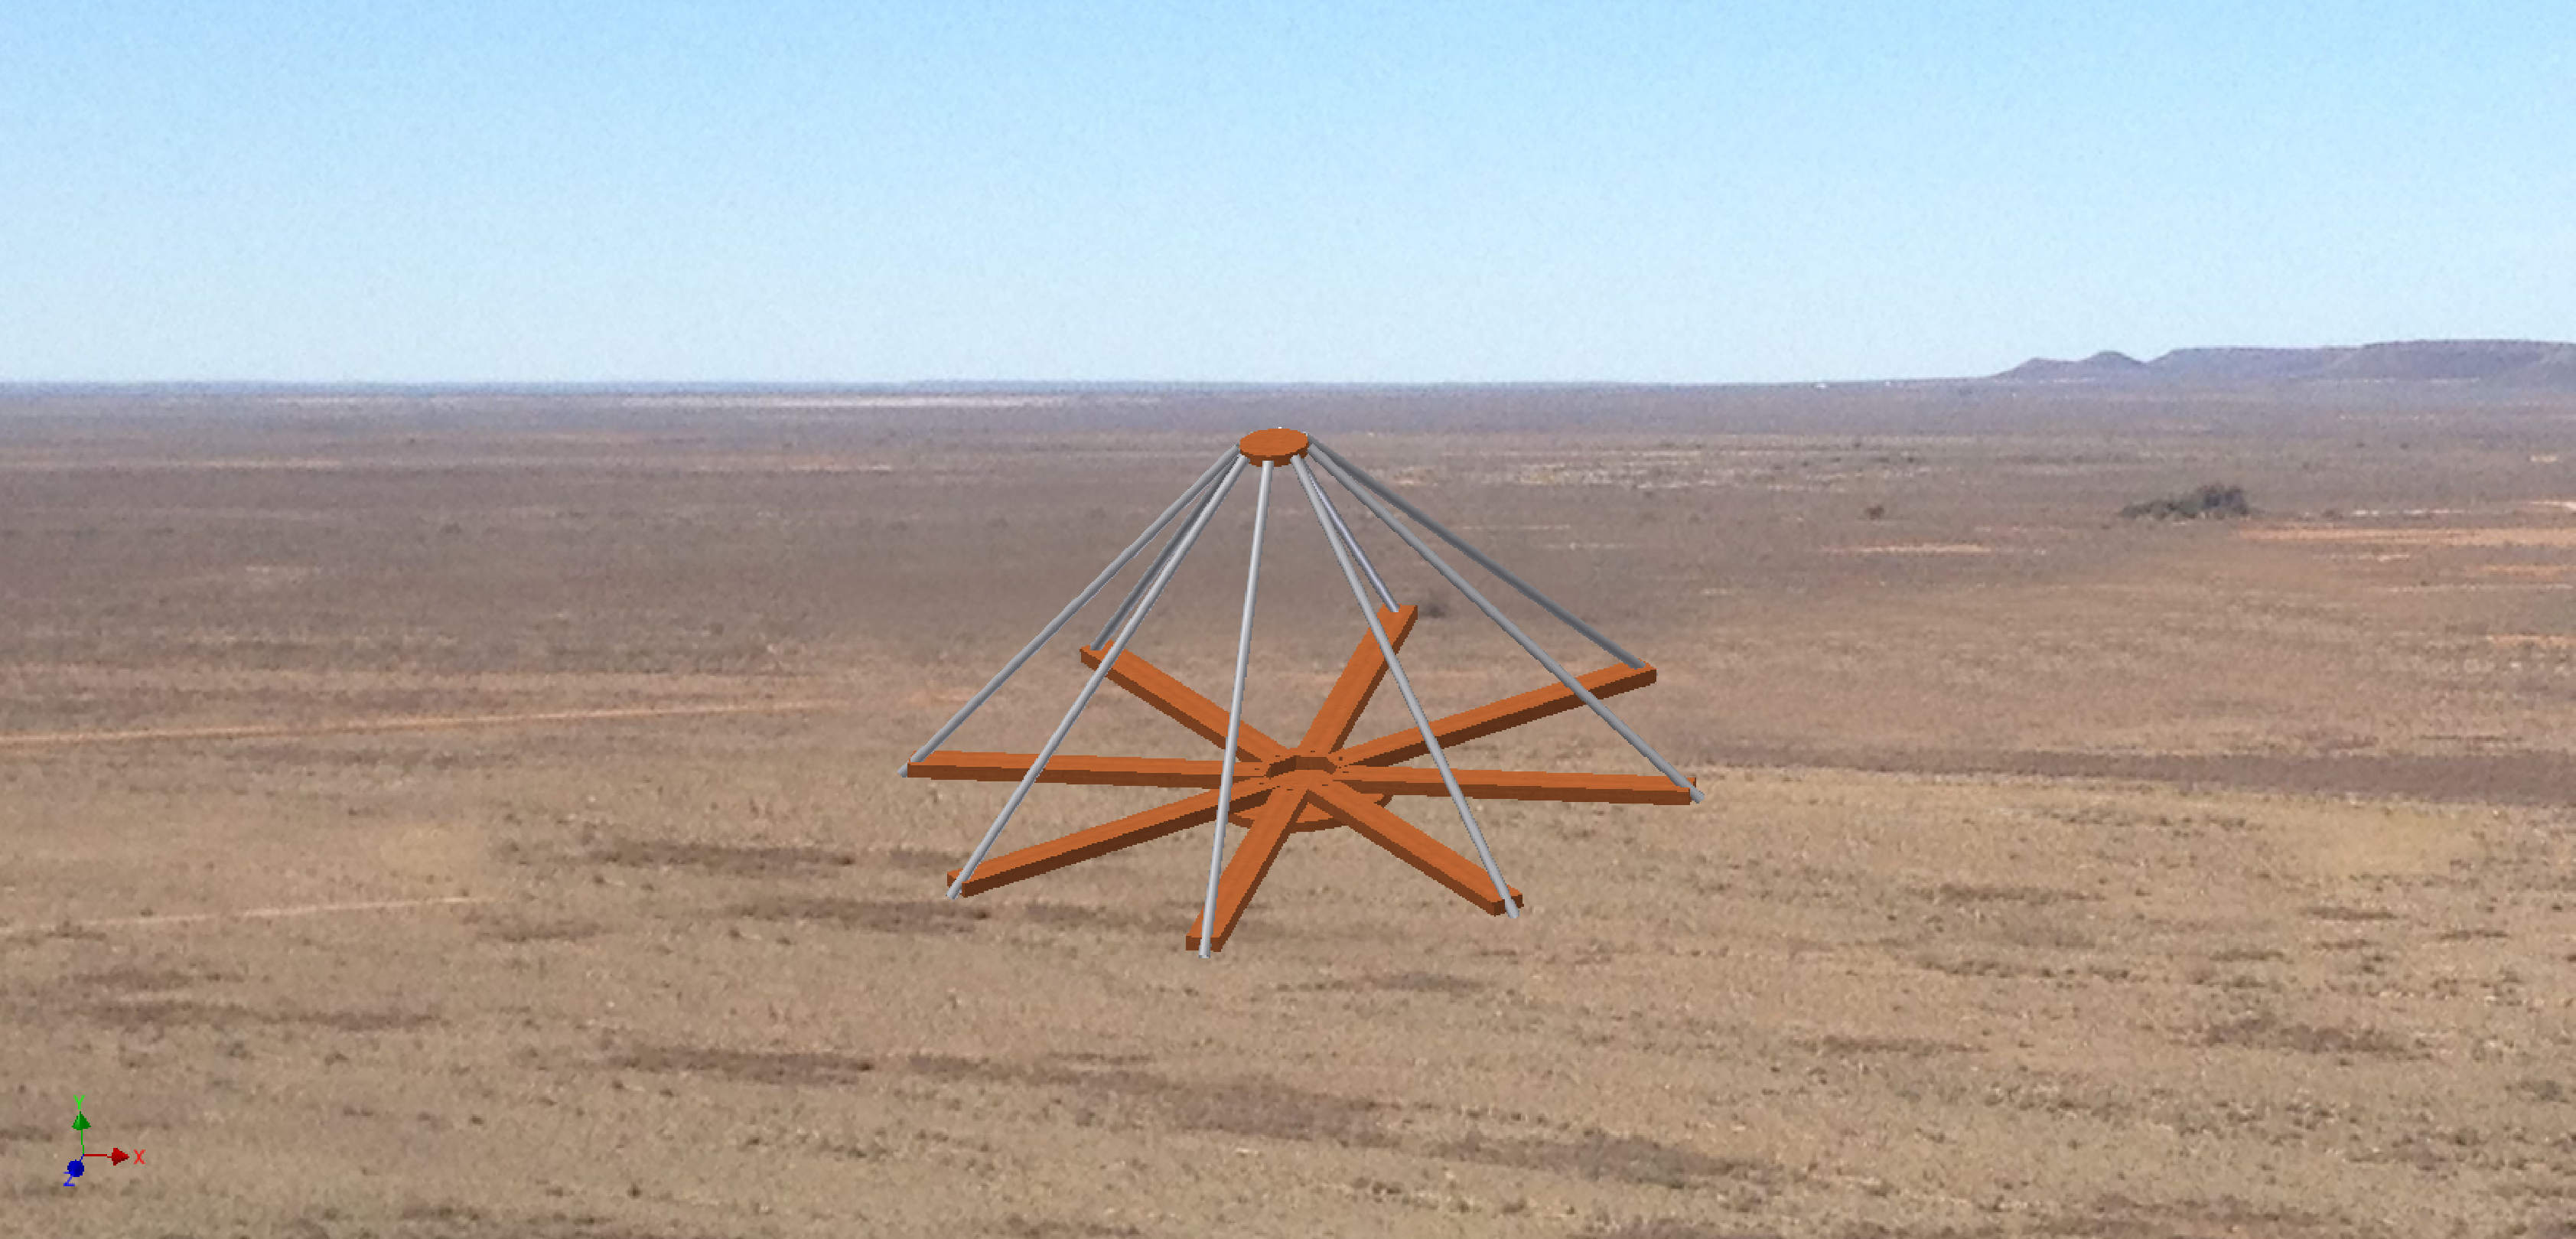
\includegraphics[width =\textwidth]{./dish_plots/splashAssembly}
	\caption{The cone structure is wrapped around with quarter inch mesh wire cloth and placed on top of the central hub centered on the vertex of the parabolic dish to reduce backlobes. This cone structure is used in the cone test, a slight modification may be applied for better backlobes reduction as suggested by the reflection measurements in the cone test. 
\label{Fig:splashcone} }
	\end{center}
\end{figure}

\subsection{hub}
The central hub has an overall diameter of 37", the inner sono tube has an interior diamater of 18", the outer sono tube has an interior diameter of 36". The launch angle of the spar sleeves is $+2.86^{\circ}$ from the inner sono tube to the outer sono tube, the supporting sleeves (botton sleeves) do not have any launch angles.


\subsection {feed suspension}
The feed suspesnsion mechanism consists of a back plane made out of wire cloth and $\frac{3}{4}$" schedule 40 white PVCs bolted on a metal hexagon, and a mast from the metal structure connecting the dipole feed to the back screen. The whole feed structure is suspended above the hub by attaching kevlar wires from the three telephone poles to the back of the metal structure. 

Each telephone pole has a reel with kelvar ropes wrapped, adjustments to feed height can be made by cranking the reels.


\subsection{material, PVC selection}
The dish structure is made out of schedule 40, white PVCs to minimize the bending effect under sunlight exposure; PVCs are subject to thermal contraction and expansion with a linear thermal coefficient of $50.4\times10^{-6}\ \frac{m}{m^{\circ}C}$.


\begin{itemize}
\item bent pipes as approximation to parabola 
\item faceting
\item shielding
\item splash cone
\item hub 
\item feed suspension (feed with mast, back screen by kevlar wire)
\item materials, PVC selection 
\item design lifetime (wood, PVC)
\end{itemize}

\section{Simulated Performance}
\label{sec:sim}

\subsection{Beam Pattern}

\begin{figure}[H]
	\begin{center}
	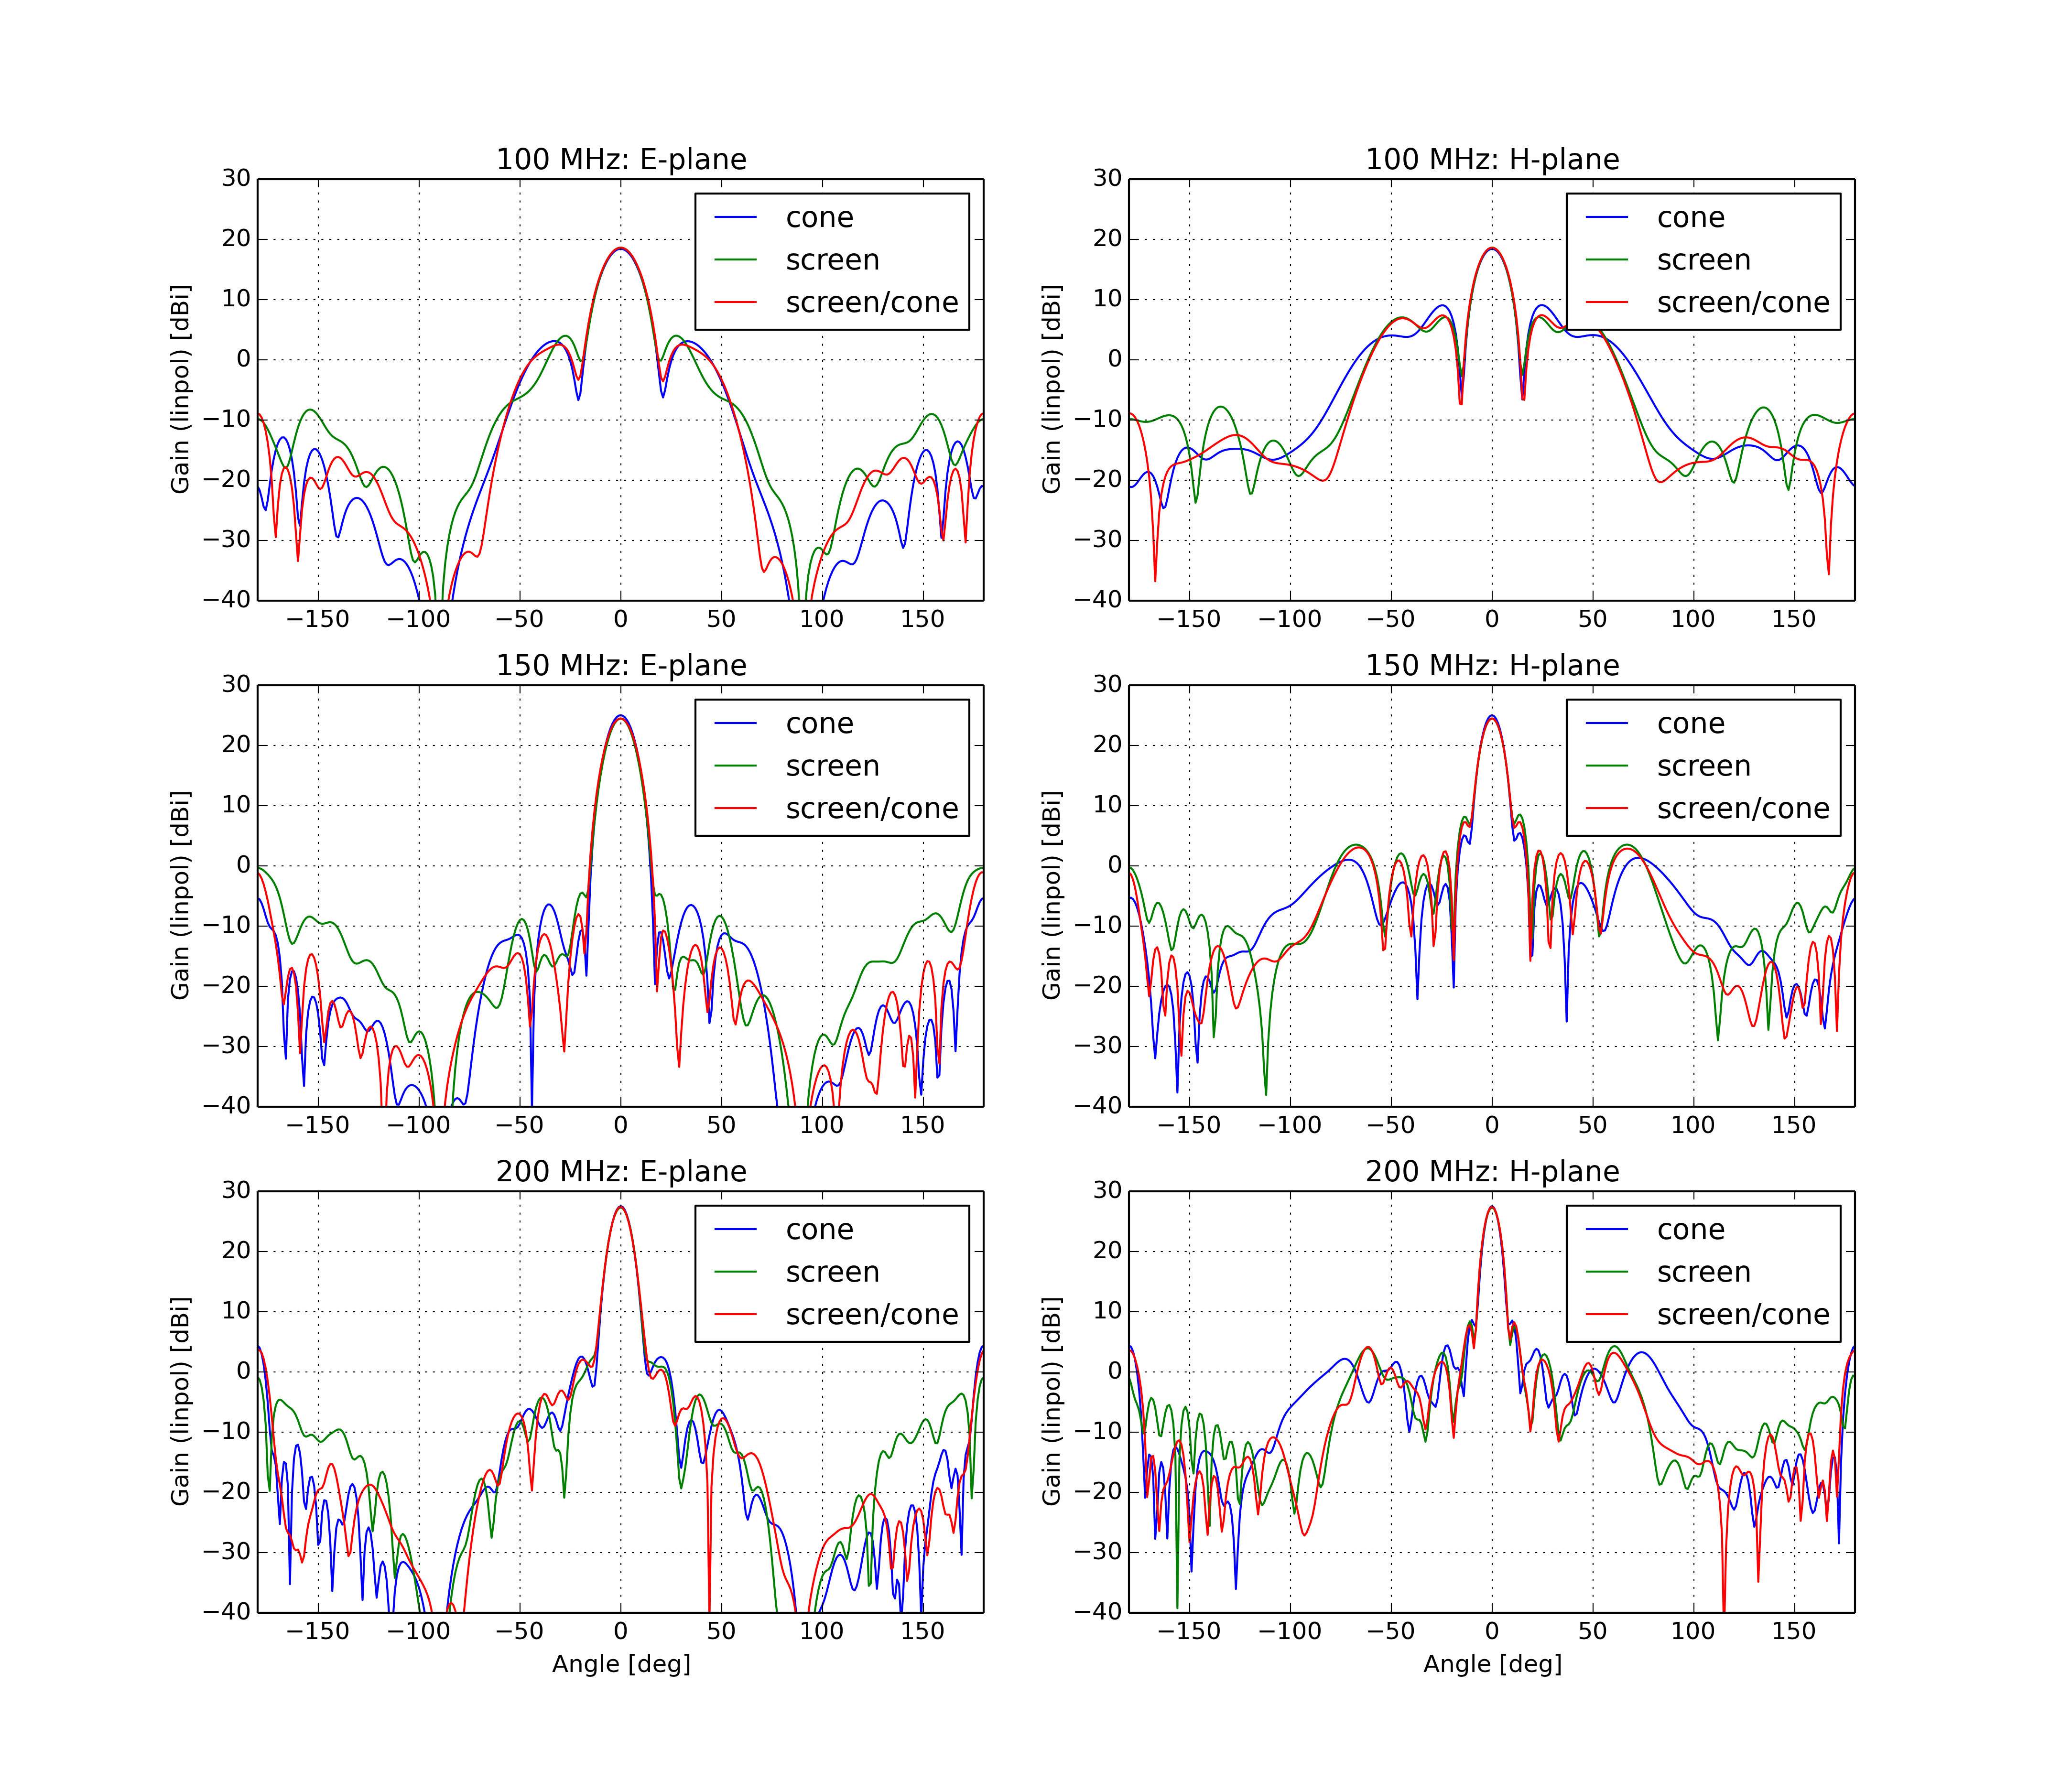
\includegraphics[width =\textwidth]{./dish_plots/Beampatterns_cone}
	\caption{THIS FIGURE SHOWS THE BEAM PATTERN 
\label{Fig:} }
	\end{center}
\end{figure}

\begin{itemize}
\item beam pattern
\item delay performance (E-M modeling)
\end{itemize}

\section{Fabrication and Deployment}
\label{sec:deploy}

\begin{itemize}
\item lessons/principles
\item process to precision to specifications on precision
\end{itemize}
\clearpage

\section{Time Domain Reflectometry}
\label{sec:reflect}
With the use of a vector network analyzer(VNA), time domain reflectometry is a technique that measures the magnitude and phase of a reflected signal (S-parameter) as function of time and frequency. The return loss of the reflection is dependent on the impedance of the device under test. The network analyzer provides
 a frequency swept signal and the inverse Fourier transform is then performed to produce reflection parameter measurements as a function of time.

When the VNA measures the S-parameters in the frequency domain, the data is measured across a pre-defined frequency range and stored at discrete points across this span. The frequency spacing between data points is proportional to the frequency span and inversely proportional to the total number of data points as shown in the following equation:
\begin{equation}
\Delta f = \frac{frequency\ span}{number\ of\ points}.
\end{equation}

The resolution in time by doing a inverse Fourier transform of the data in frequency is inversely proportional to the frequency resolution:
\begin{equation}
\Delta t = \frac{1}{\Delta f}.
\label{Eqn:res}
\end{equation}
Time domain reflectometry(TDR) is carried out with the feed as the device under test after the mesh panels are installed. In this application, time domain reflectometry measures the reflections on the dish as a function of time as a result of impedance mistmatch between the feed electronics and the sky signal. The characteristic impedance of the output signal from the feed generated from the vector network analyzer and transmission coaxial cable is $50 \Omega$. With the use of a 4:1 passive balun at each polarization, the signal at the feed has a characteristic impedance of $200\Omega$ and that of the free space is $120\pi\Omega$. 

Each polarization is connected to a port on the vector network analyzer, the time axis represent the physical distance as the signals propagate along the transmission cables. The physical distance of can be related to the time axis using:
\begin{equation}
D = \frac{t}{2}v_{fac}c,
\end{equation}
$t$ is the round trip travel time as recorded as the time data.
The VNA is calibrated at the end of the cables connecting the baluns, hence the velocity factor in the measurements can be taken as $1$, resulting the speed of propgation to be the speed of light $c$. As a rule of thumb,  $1$ ns is equivalent to $1$ ft in free space from the passive baluns. The expected reflection from simulation and mathematical derivation is -$60$dB by $2$ reflections between the focal point and the vertex. The designed focal length of the dish is $4.5$m, $2$ times of reflection (i.e. $4$ crossings attenuation) corresponds to $59.0$ ns in time domain.
\subsection{Choice of Hardware}
The same feed as PAPER is used in this prototype , consisting a half-wavelength dipole for each polarization and a 4:1 passive balun is attached to the dipole through a mating board for each polarization. The other end of the $50\Omega$ coaxial cables connect the baluns to the ports of a VNA for time domain reflectometry. The LMR400 coaxial cables of length 10 m has a signal attenuation of $\sim$0.5 dB over 10 m at 150 MHz. The Aglient ES8753A is being used as the VNA to carry out the TDR measurements, the system dynamic range is 100 dB at 16 MHz to 3 GHz and the directivity is 55 dB at 300 kHz - 1.3 GHz, where the frequency range of interest is 50 MHz - 1 GHz. 

\subsection{Calibration of VNA}
Calibration is performed prior to taking measurements to eliminate the systematic effects caused by cables, adapters, and connectors. Performing calibration at the end of the cables shifts the reference plane to the SMA connectors of the cables that are connecting the baluns with zero phase, zero loss and zero mistmatch; as such, the measurements taken are showing only the effects of the feed and baluns under different configurations. The full two port calibration is done by attaching the calibration standards (SHORT, OPEN, LOAD, and THROUGH) to the end of the $50\Omega$ cables, the VNA calculates the correction coefficients and applies the coefficients subsequently to each measurements. The calibration coefficients includes offset delay, capacitance in the form of a fourth order polynomial, inductance as a fourth order polynomial, offset loss as resistance per second, and offset characteristic impedance. 

A SHORT standard calculates the offset delay, offset loss, and specifies the inductance coefficients $L_0$ through $L_3$ to model the phase shift caused by the residual inductance in the standard as a function of frequency by fitting a forth order polynomial. An OPEN standard calculates offset delay, offset loss, and specifies the capacitance coefficients $C_{0}$ through $C_{3}$ to model the phase shift due to fringing capacitance as a function of frequency by fitting a forth order polynomial. The offset delay is the one way propagation time that can be obtained from speed of light in free space, the physical length and the permittivity constant of the cable material; the offset loss is caused by the skin effect of offset coaxial type standards. During the calibration process, the SHORT standard and OPEN standard are off by $180^\circ$; the reflection coefficients should be $1$ (0 dB) at $0^\circ$, and $1$ at $180^\circ$ at all frequencies for OPEN standard and an ideal zero-length short respectively. A perfect LOAD standard should have a reflection coefficient of $0$ as the characteristic impedance $Z_o$ matches the specfied impedance on the network analyzer. The effect and its significance is shown in Figure \ref{Fig:calibration}. 

\begin{figure}[H]
	\begin{center}
	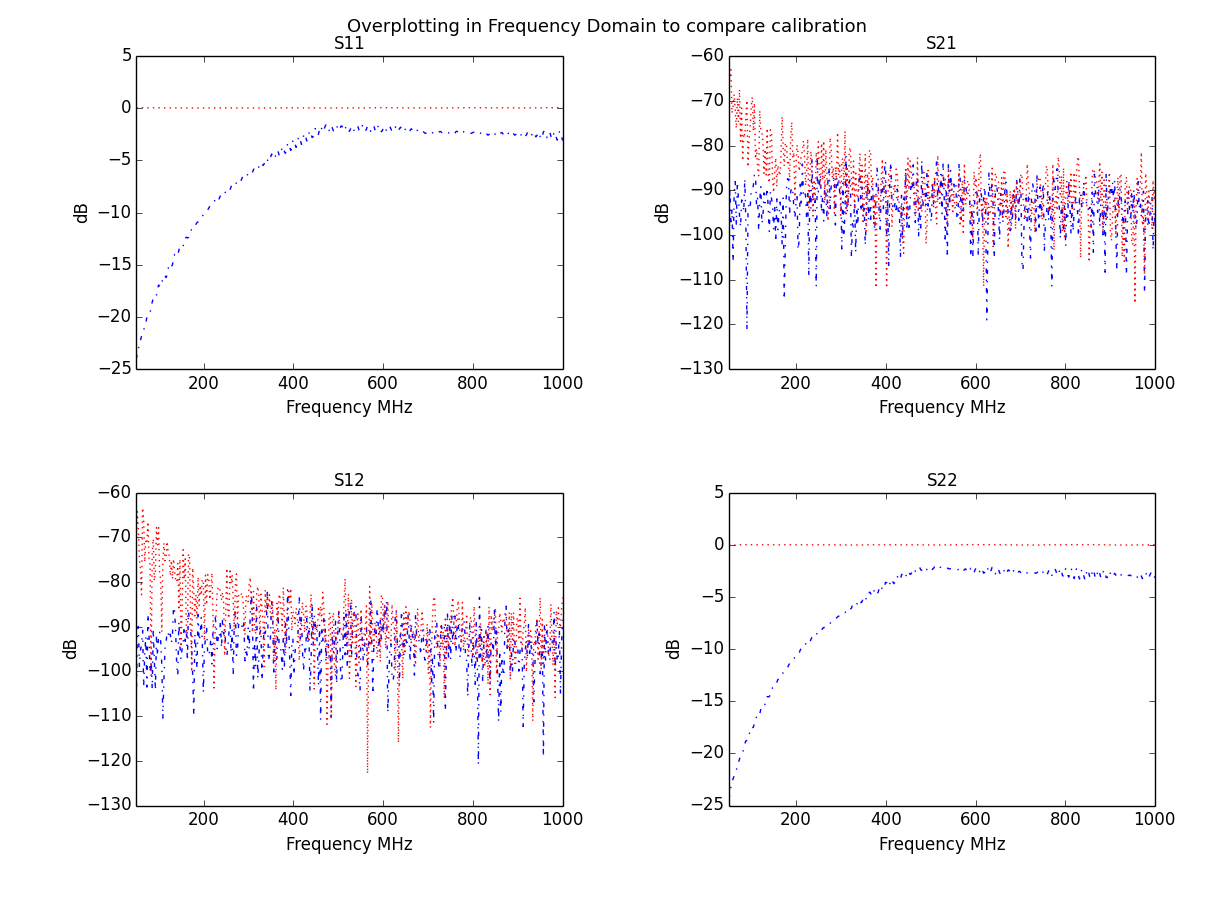
\includegraphics[width =\textwidth]{./reflectometry_plots/Calibration_open}
	\caption{The reflection and tramission paramters of the full 2-ports are plotted as a function of frequency to show the significance of applying standard calibrations prior to taking measurements. The blue curves represent the uncalibrated results, and the red curves represent the calibrated results of open ends at the far end of the cables that are connected to the network analyzer. }
\label{Fig:calibration} 
	\end{center}
\end{figure}
\clearpage
\subsection{Configurations}
The measurements are taken with 401 data samples between 50 MHz to 1 GHz, giving a time resolution of 1.05 ns; each set of data is averaged by 16 measurements for higher SNR. The first test being carried out is by varying the feed height above the vertex, and the second test is by placing a splash cone on the central hub centered on the vertex of the parabolic dish. The feed height test was carried out at three different heights above the dish: $67"$, $10'3.5"$, and $14'0.5"$ to verify the effect of reflection as a function of time delay which is directly related to the travelled distance of a signal and the number of crossings attenuation. The cone test was carried at a distance $14' 6"$ above the vertex to investigate the backlobes of the antenna and the effectiveness of reducing the backlobes by placing the splash cone structure as shown in Figure \ref{Fig:splashcone}.
\subsection{Window Functions}
To deal with real-life situations of a finite bandwidth which results in spectral leakage in time domain,  the Kasier-Bessel window is applied to the frequency domain data prior to performing the inverse Fourier transform in order to increase the dynamic range of the measurements in time domain by reducing the sidelobes; the disadvantage however, is the widening of the pulse width between data points hence reducing the time resolution , hence the resolution equation in Equation \ref{Eqn:res} is an approximation. As shown in Figure \ref{Fig:window}, the spectra features are emphasized by multiplying a window function to the frequency response prior to performing the inverse Fourier transform to time domain. 
\begin{figure}[H]
	\begin{center}
	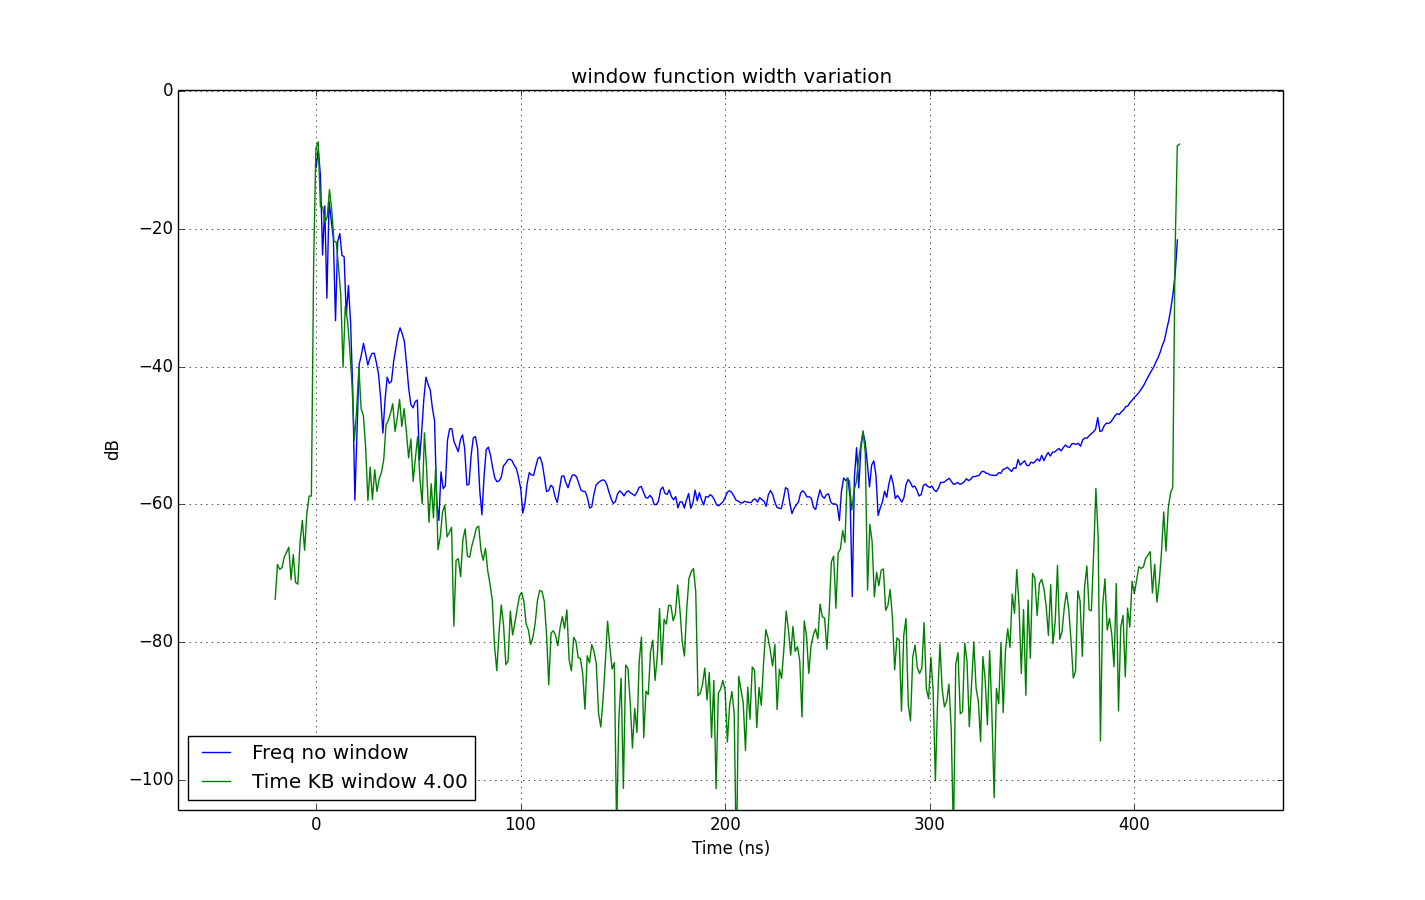
\includegraphics[width =.8\textwidth]{./reflectometry_plots/win_nowin}
	\caption{If a window function is used to weigh the spectrum prior to performing an inverse Fourier transform, the sidelobes are reduced as shown by the green curve which is weighted by a Kaiser-Bessel window with $\beta = 4.0$ before the IFT.
\label{Fig:window}}
	\end{center}
\end{figure}

\clearpage
The sidelobes can be reduced thereby increasing the dynamic range in a spectrum by varying the width or the $\beta$ value of a Kaiser-Bessel window as demonstrated by Figure \ref{Fig:windowwidth} and more discernible in the time range 200-300 ns. Some of the features are suppressed near 40 ns when $\beta = $8.6(blue) is used compared to when $\beta = $4.5(red) or $\beta = $4.0(green) is used. The strong reflection peak to the left of 40 ns is caused by impedance mismatch along the signal path in the connectors on the balun and the mating board, and a steeper roll off, hence the suppression is resulted when weighted with a larger $\beta$ value. For this reason, we employed $\beta = $4.5 in the analysis.

\begin{figure}[H]
	\begin{center}
	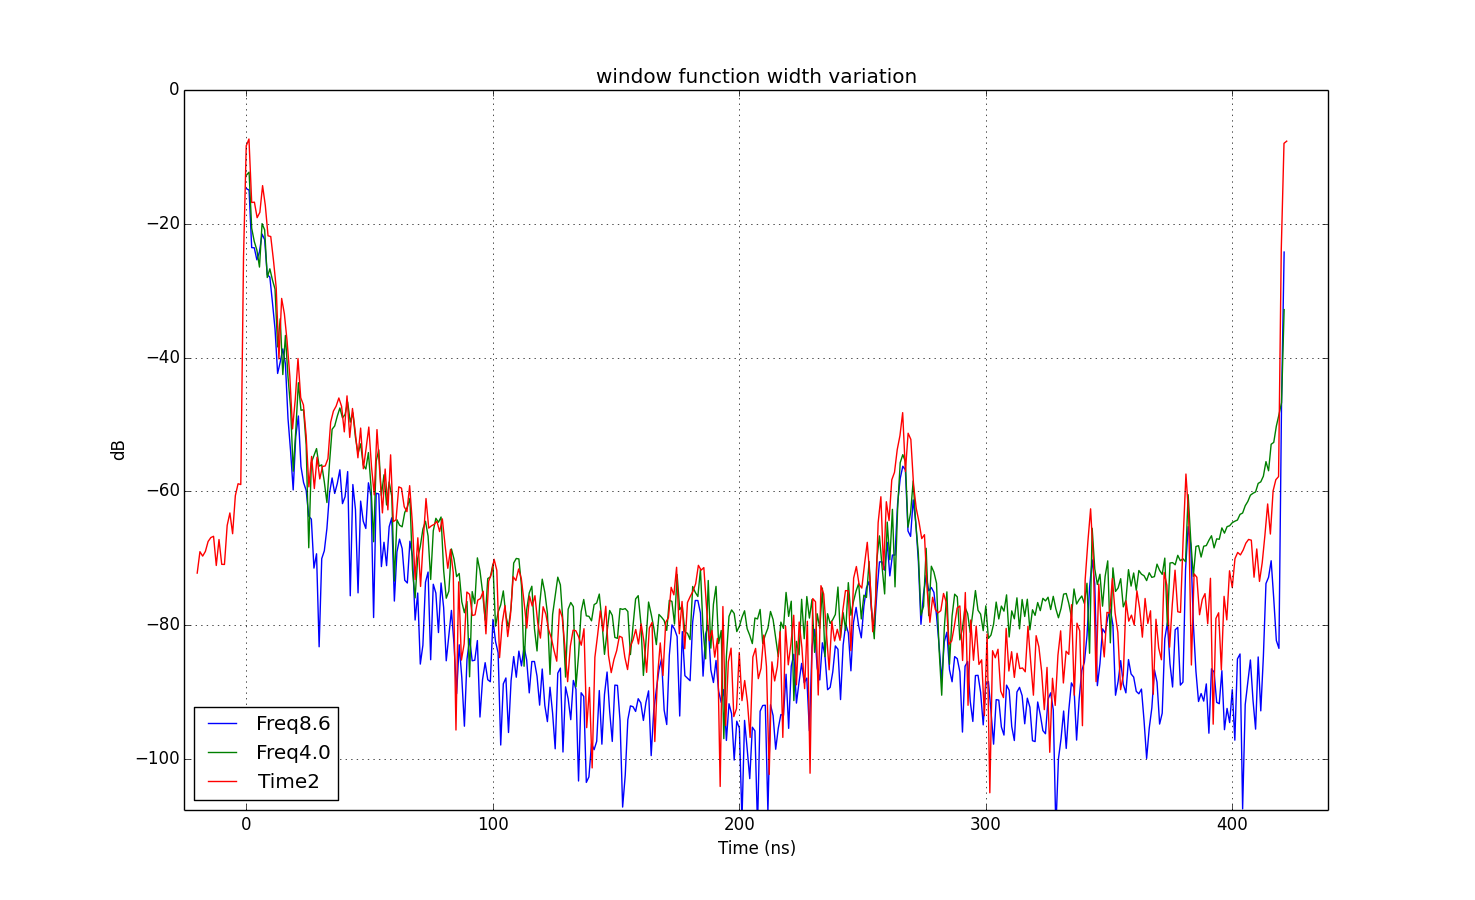
\includegraphics[width =.8\textwidth]{./reflectometry_plots/window_width_variation}
	\caption{$\beta$ values of 8.6, 4.5, and 4.0 in a Kaiser-Bessel function are applied to the frequency spectrum prior to performing the inverse Fourier Transform. Since a $\beta$ value of 8.6 suppressed some of the features as a result of the strong reflection peaks nearby, $\beta = $4.5 is used for the analysis to ensure high dynamic range as well as retaining spectrum features to be observable.
\label{Fig:windowwidth}}
	\end{center}
\end{figure}
\clearpage
\begin{itemize}
\item reflectometry 
\item hardware 
\item calibration of the good
\item feed height test
\item configurations
\item window function used in delay transform
\end{itemize}

\section{Results}
\label{sec:results}
\subsection{Delay Spectrum for Configurations}


The peaks associated with signal reflections from the vertex of the parabolic dish are relatively lower than those resulting from the adapters, electronic parts and surrounding environment. 

All the traces in Figure \ref{Fig:moutain} show that there are two large peaks representing the reflection from the moutains nearby, one at xxx ft another at xxx ft. Some traces in the figure are measured while the dish was not on the dish, ~ xxx ft from the dish and those two peaks resulting from the moutains shifted in time accordingly.


\begin{figure}[H]
	\begin{center}
	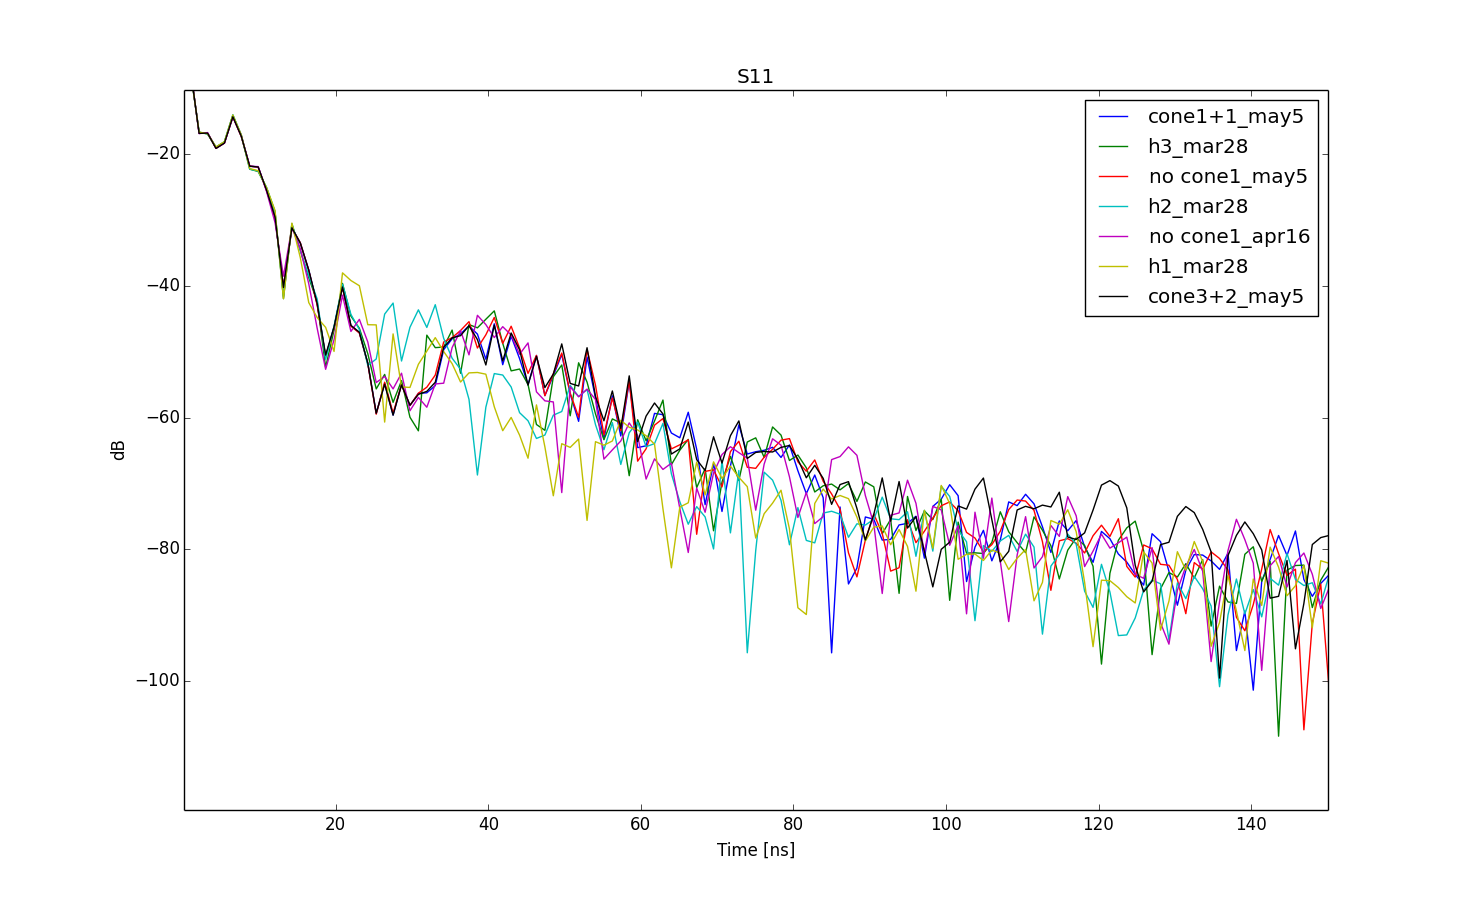
\includegraphics[width =.7\textwidth]{./reflectometry_plots/configcompare10-150ns}
	\caption{Shows the reflection parameter S11 plot with the height tests, cone test, can see height test changed the delay, each configure is plotted on different plots below.
\label{Fig:} }
	\end{center}
\end{figure}

From these measurements, the peaks associated with the connectors and surrounding enviornment are static as these components were the invariants during the measurements. 
\begin{figure}[H]
	\begin{center}
	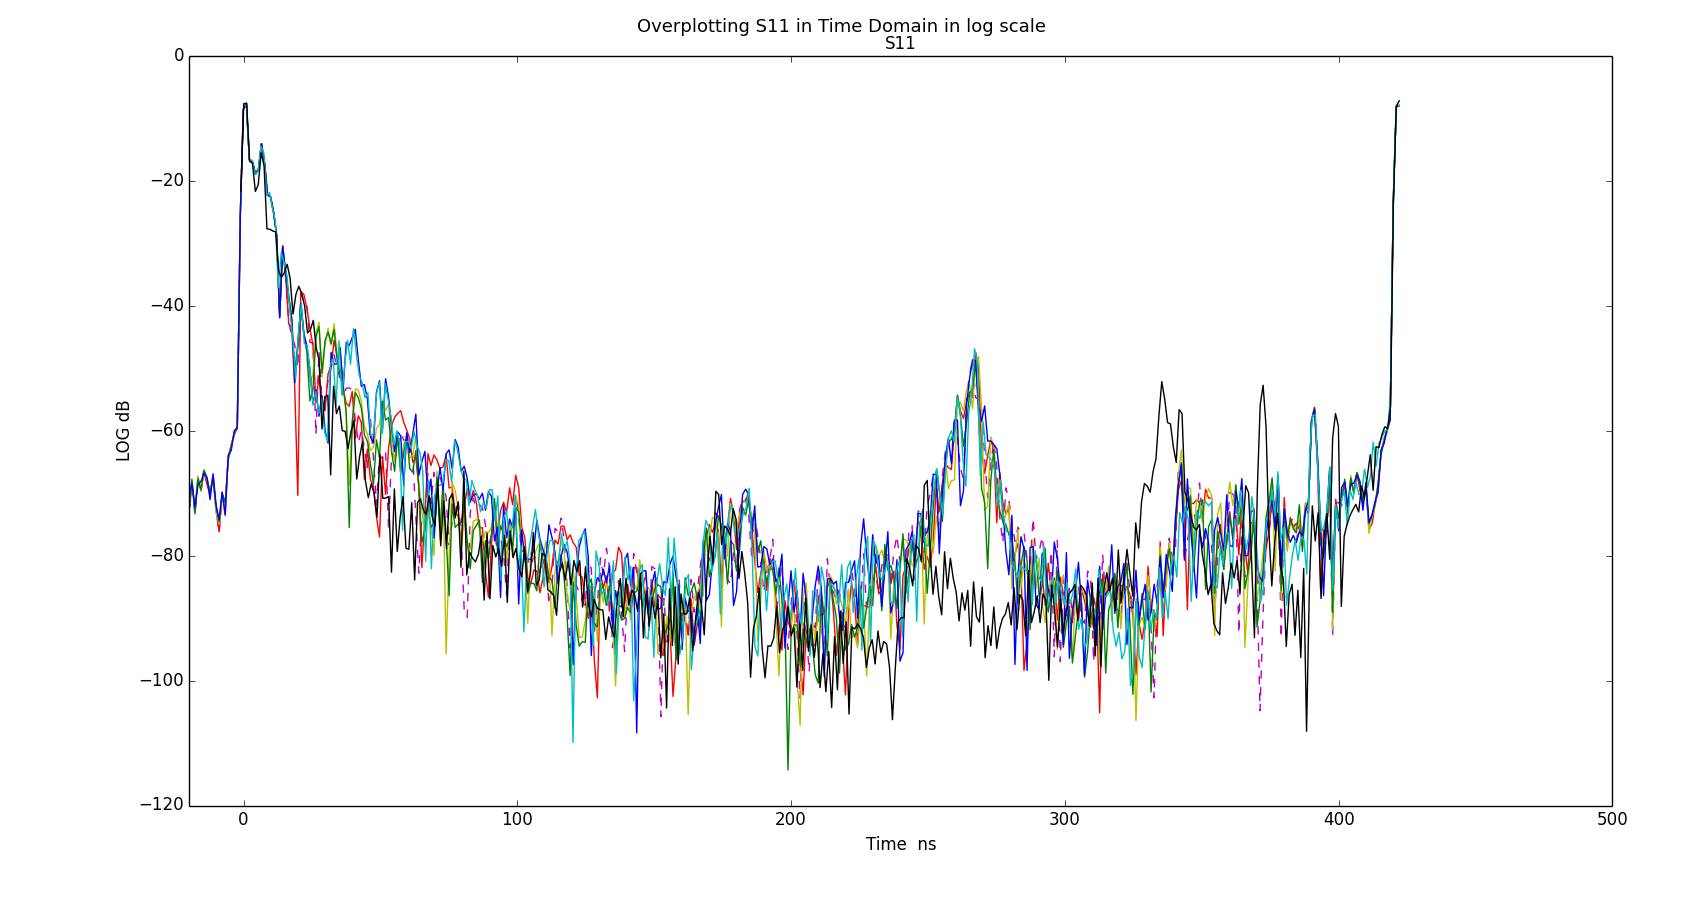
\includegraphics[width =.7\textwidth]{./reflectometry_plots/Mar28/s11all-mar28mix17set1}
	\caption{Shows height tests on dish, test not on dish, shows bump is reflection due to surroundings. mountain bumps ~ 60' - 80'
\label{Fig:moutain} }
	\end{center}
\end{figure}


results@ height 14' 6"
Dish with and without cone, with screen covering panel A, B

\begin{figure}[H]
	\begin{center}
	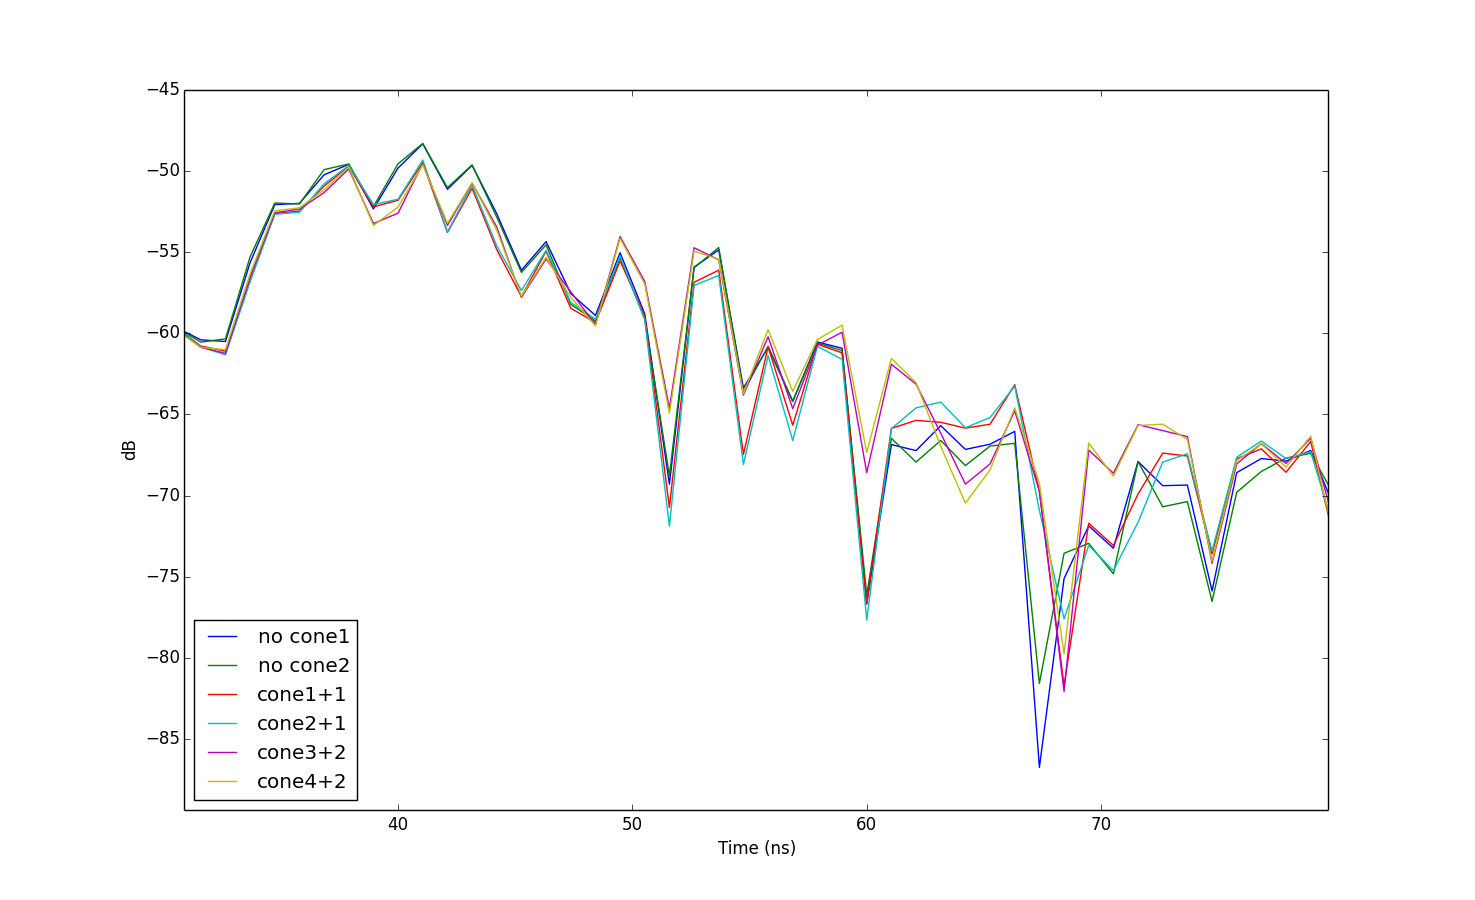
\includegraphics[width =.7\textwidth]{reflectometry_plots/May5/S11_1st2nd_refl}
	\caption{Shows cone VS no cone, combine 2 plots above, apparent difference cone make, but needs redesign for better backlobe minimization as seen from ~45ns.
\label{Fig:conetest} }
	\end{center}
\end{figure}

========
dish different heights
h1 = 67"
h2 = 10'3.5"
h3 = 14'0.5"
Figure \ref{Fig:height_test} also shows the time domain response when the feed is positioned XXX above the vertex.
There is also a noticeable increase in the peak amplitude associated with the feed when the plate is moved closer to the central hub. 
This increase in peak amplitude is due to the reduction in space loss as the signal now propagates over a shorter distance.


The first reflection as plotted around 20-50 ns depending on the height of the feed; as it is moved
closer and further, the measured time domain response shows an equivalent time shift in the peak. 

\begin{figure}[H]
	\begin{center}
	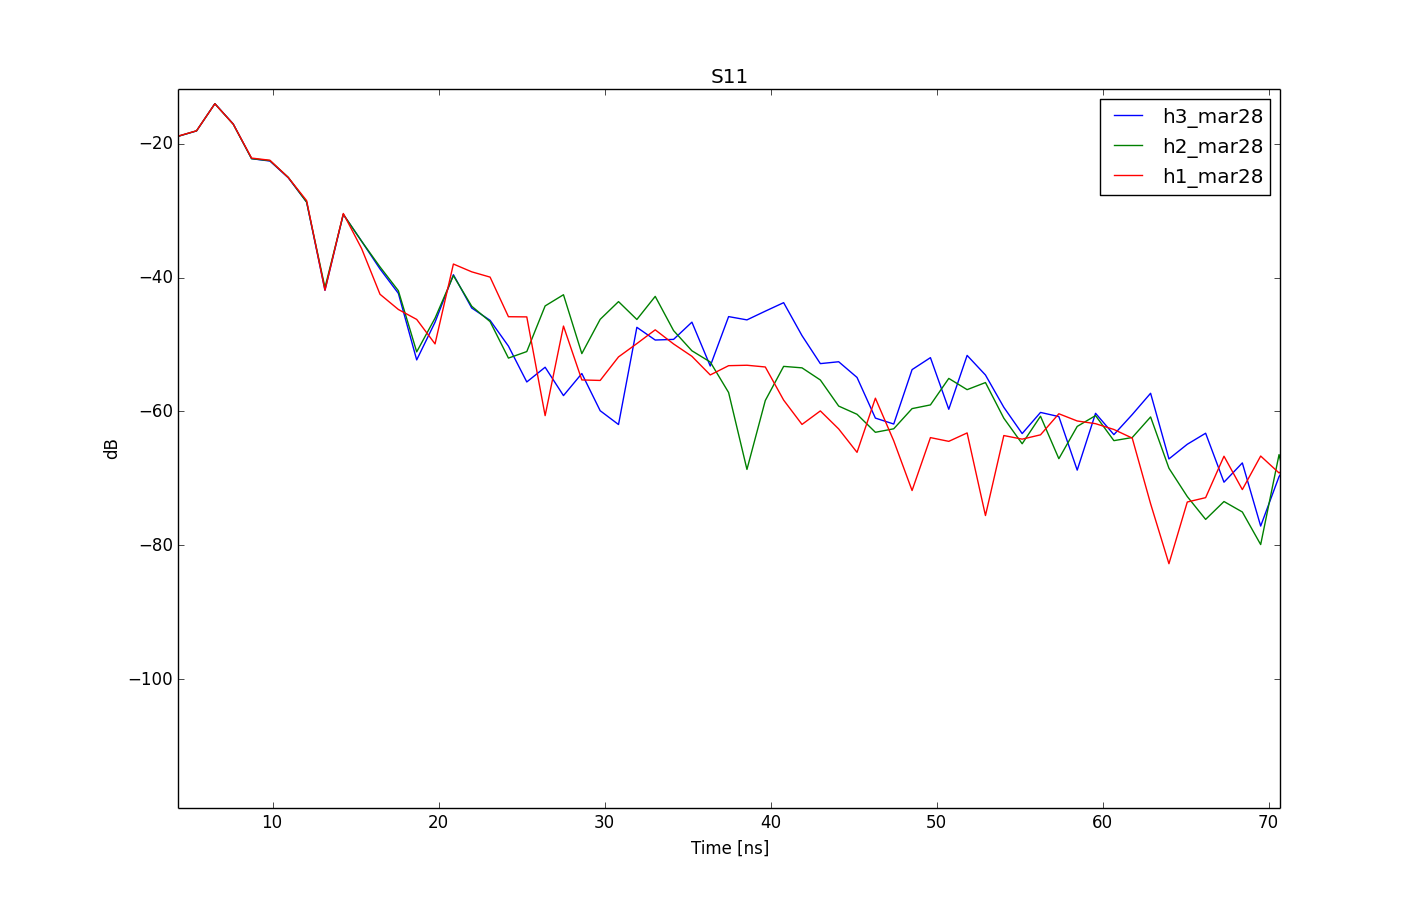
\includegraphics[width =.7\textwidth]{reflectometry_plots/Mar28/height_test_zoom}
	\caption{height test showing delay depending on feed height
The red curve has highest peak amplitude, followed by the green curve and lastly the blue curve, each increases by 4' of the preceeding color curve. The peak amplitude varies inversly as the height of the feed. Blue shows similar amplitude as green since blue is at the focal length of the parabolic surface.
\label{Fig:height_test} }
	\end{center}
\end{figure}



\subsection{Cone test}


For the case without the splash cone, shown in Figure \ref{Fig:conetest}, cone helped on reduce backlobe

\clearpage
\subsection{RFI investigation}
To measure the spectra of the sky with the prototype, the dipole element is connected to the PAPER active balun which amplifies the signals from both polarization by XX dB and outputs $75\Omega$ signals into the PAPER receiver which contains two 100-200MHz bandwidth filters, and outputs $50\Omega$ signals after amplification. The $50\Omega$ signals travel along the LMR 400 cables to the Agilent E4407B spectrum analyzer. The spectra are taken with 401 data points, ranging from 100-200MHz, and 50 measurements are averaged to improve the SNR, the resolution bandwidth is specified to be 1 MHz with 0 dB attenuation, and the resulting spectra has a resolution of 0.25 MHz.

Cygnus A, a radio bright source is at right accension $19h59m28s$ and declination $+40^\circ44'02"$ and the dish is located at $+37.98^\circ$ latitude, and $-122.19^\circ$ longitude. Cygnus A, hence is an ideal source for the sky test as it transits at night time during the summer when observations are carried out. Three spectra shown in Figure \ref{Fig:RFI} are taken at different times in a day: daytime, before and during the transit of Cygnus A in our beam during the nighttime.

\begin{figure}[H]
	\begin{center}
	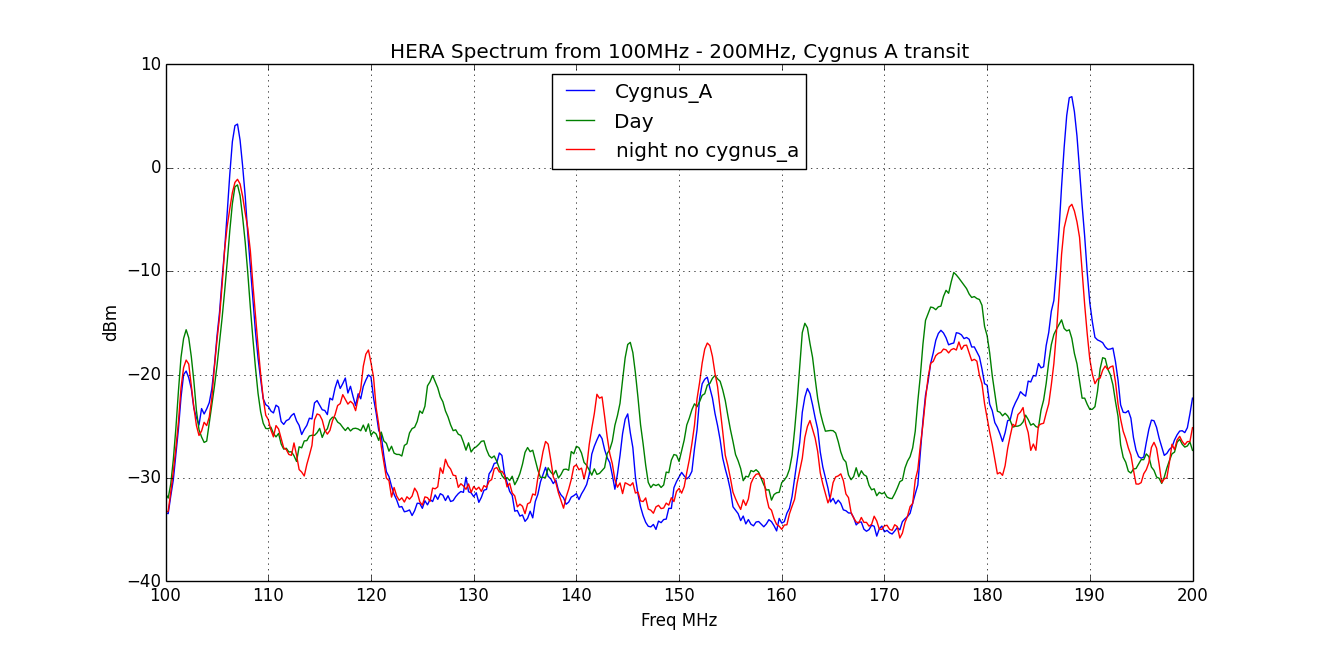
\includegraphics[width =.8\textwidth]{spectra_plots/transit,day,night_match-yaxis.png}
	\caption{Three spectra taken at different times in a day spanning the frequency range from 100 MHz to 200 MHz. Radio stations and TV broadband channels are the major RFIs in the vicinity of our dish. During nighttime, as shown by the blue and red curves, the beam pattern can be studied by observing the power of a radio bright source throughout the night in those narrow channels with minimal RFIs.
\label{Fig:RFI}}
	\end{center}
\end{figure}

Spectra in Figure \ref{Fig:narrowchannels} are taken at nighttime, approximately 4 hours before Cygnus A transits within the beam to ensure uncontaiminated frequency channels can be effiectively identified. As the resolution bandwidth is reduced from 1 MHz to 1 kHz and the averaging number of measurements is reduced to 0, channels with minimal RFIs are identified as 120-130 MHz, 155-160MHz, 165-175MHz and color plotted as green, red, and cyan respectively in Figure \ref{Fig:narrowchannel}.
\begin{figure}[H]
	\begin{center}
	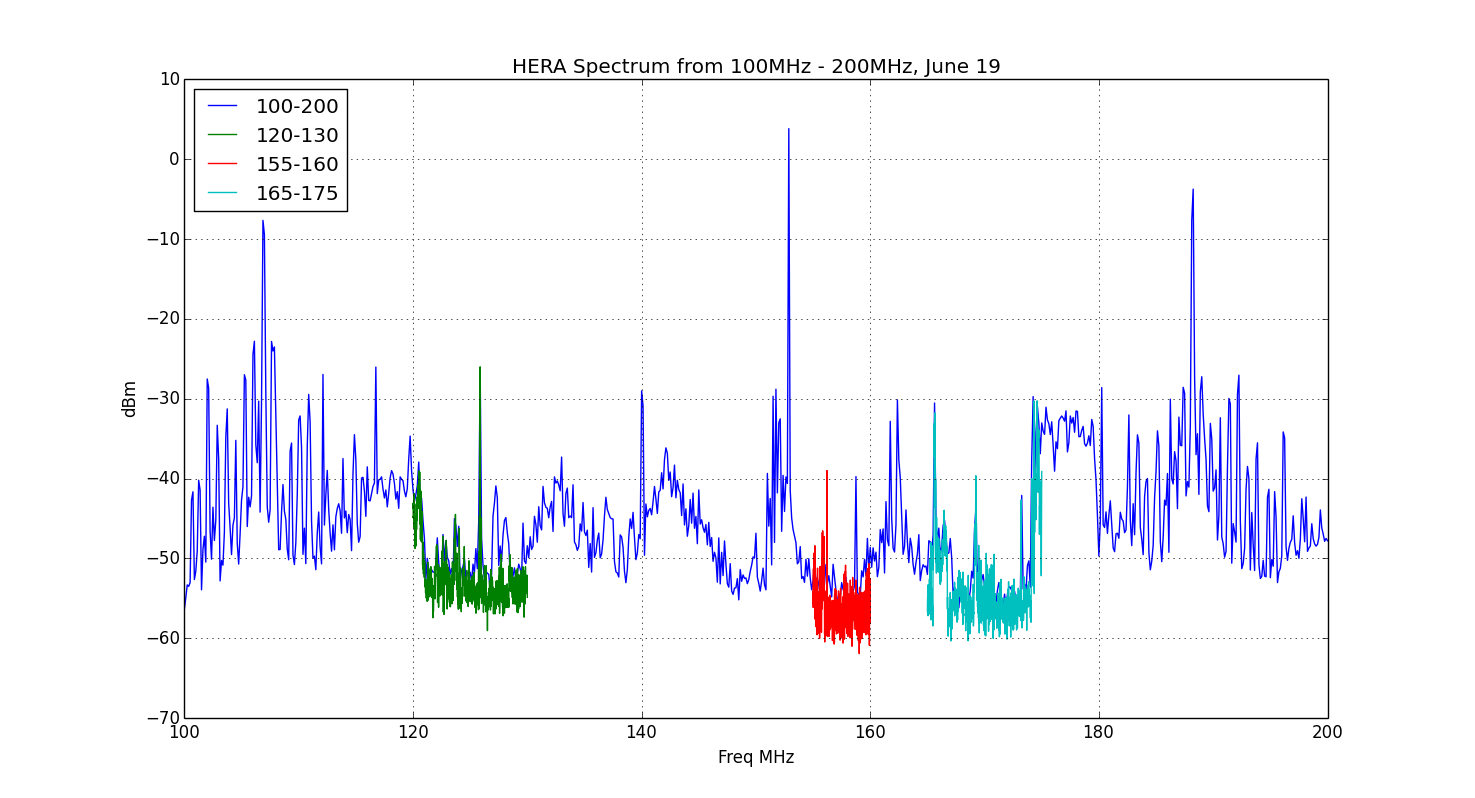
\includegraphics[width =.8\textwidth]{spectra_plots/all_channels}
	\caption{The narrow channels with minimal RFIs are identified as 120-130 MHz, 155-160 MHz, and 165-175 MHz. The power in dBm are lower than the spectra shown in Figure \ref{Fig:RFI} as the resolution bandwidth is reduced from 1 MHz to 1 kHz.
\label{Fig:narrowchannels} }
	\end{center}
\end{figure}
\clearpage

Spectra are taken in those frequency channels every $10\pm2$ minutes throughout a night as Cygnus A rises and transits across the beam. Figure \ref{Fig:120130allnight}, and \ref{Fig:165173allnight} show that within these narrow channels that were identified according to the 100-200MHz spectra, RFIs were present occassionaly throughout the observing night; hence, narrower channels within the spectra are extracted to calculate the power as a function of altitude and local sidereal time.

\begin{figure}[H]
	\begin{center}
	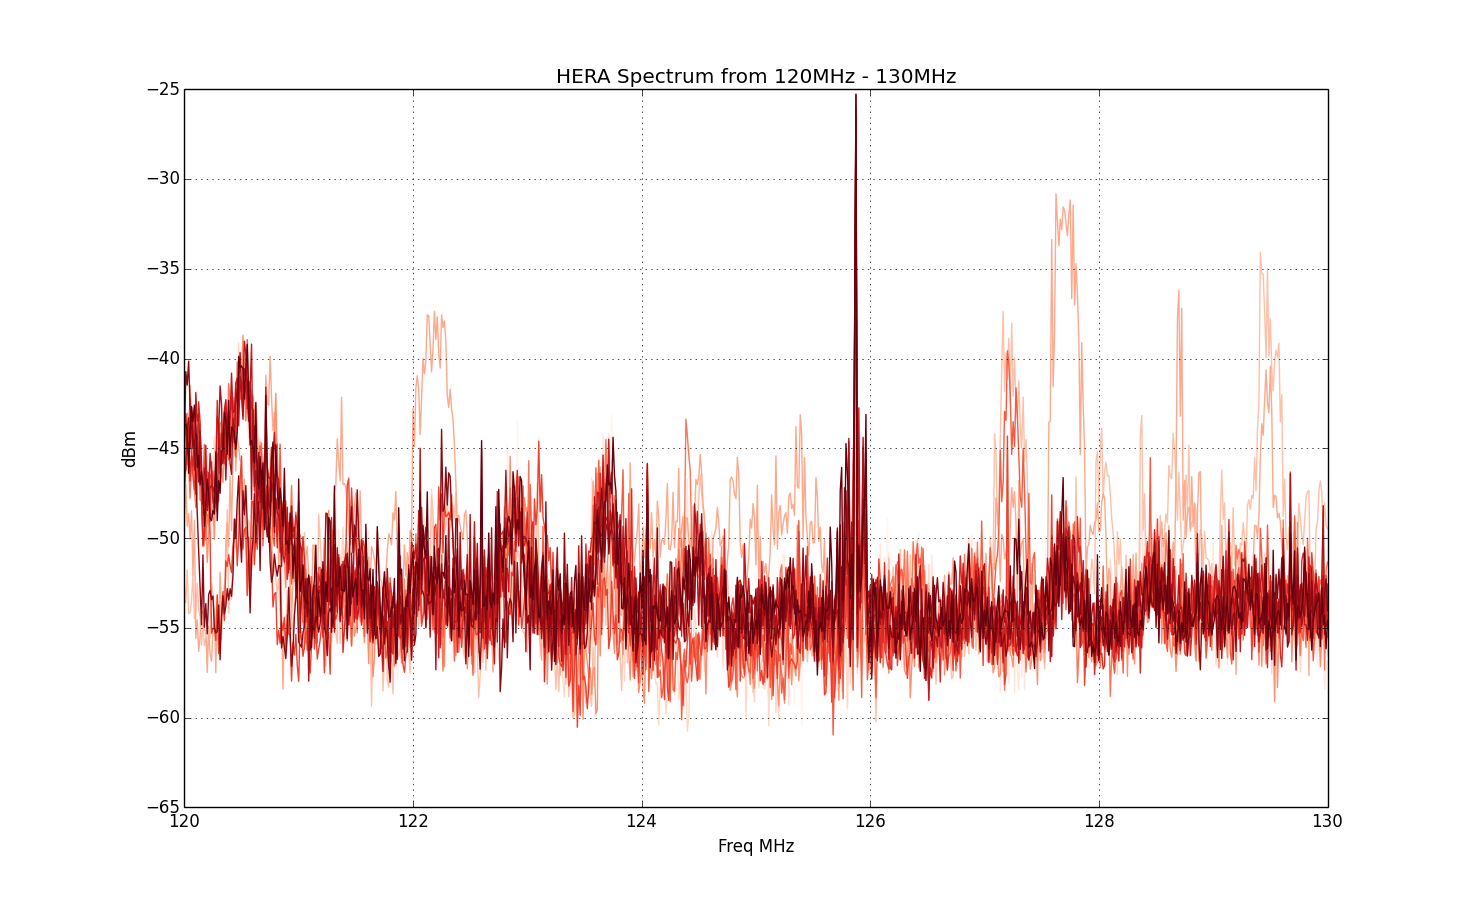
\includegraphics[width =0.85\textwidth]{spectra_plots/120130allnight}
	\caption{Here, the spectrum running from 126 MHz to 127 MHz is the quiet region within the 120-130 MHz channel that was chosen according to the 100-200MHz nighttime spectrum shown in Figure \ref{Fig:narrowchannels}.
\label{Fig:120130allnight} }
	\end{center}
\end{figure}

\begin{figure}[H]
	\begin{center}
	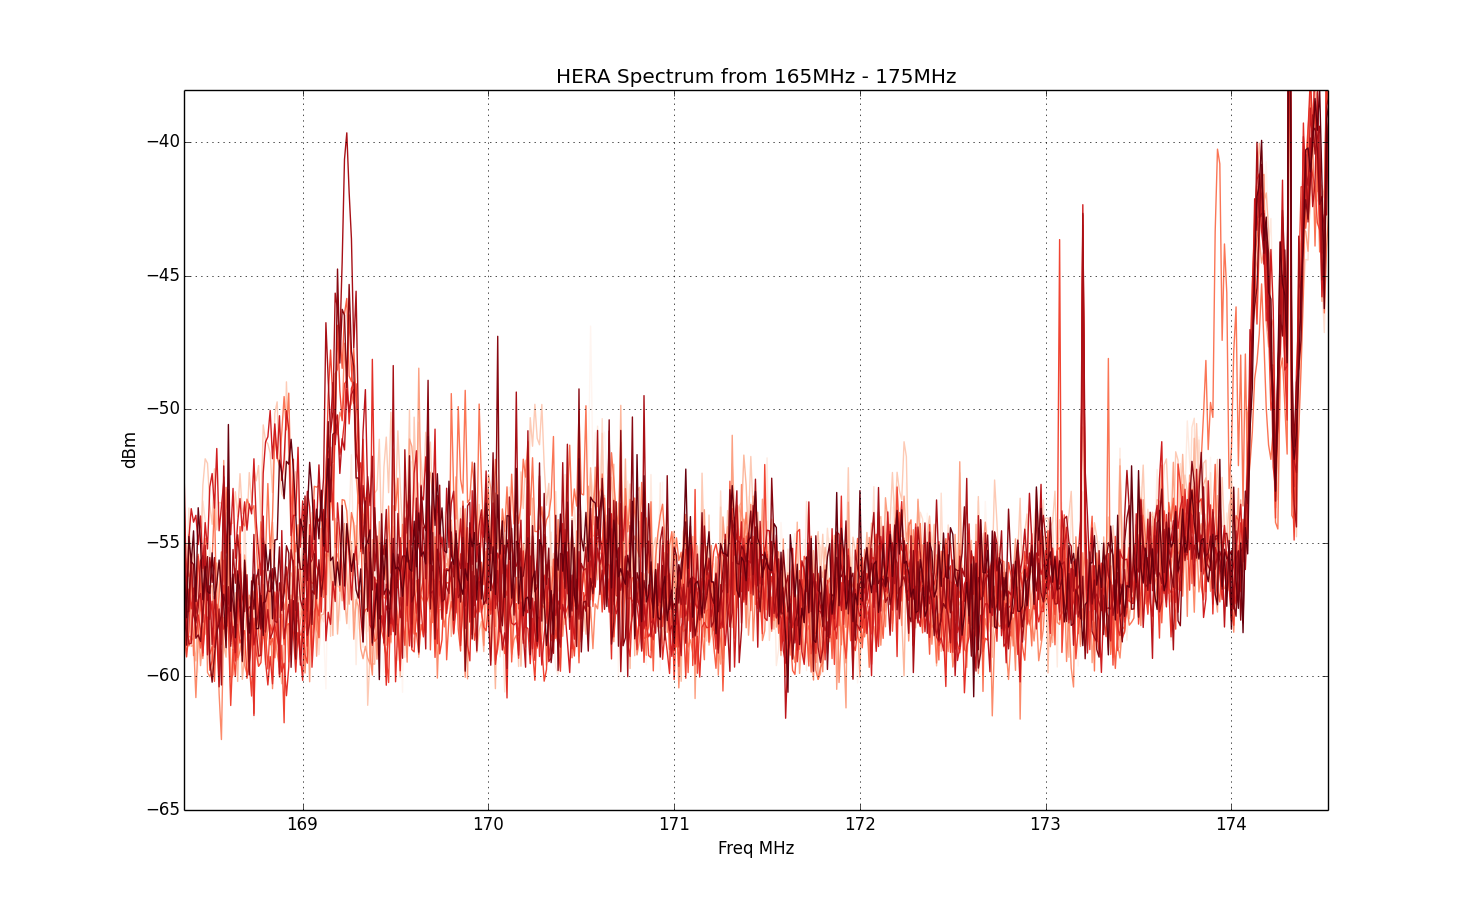
\includegraphics[width =0.85\textwidth]{spectra_plots/clean171173}
	\caption{Here, the spectrum running from 171 MHz to 173 MHz is the quiet region within the 165-175 MHz channel that was chosen according to the 100-200MHz nighttime spectrum shown in Figure \ref{Fig:narrowchannels}.
\label{Fig:165175allnight} }
	\end{center}
\end{figure}

blah blah blah blah blah
\begin{figure}[H]
	\begin{center}
	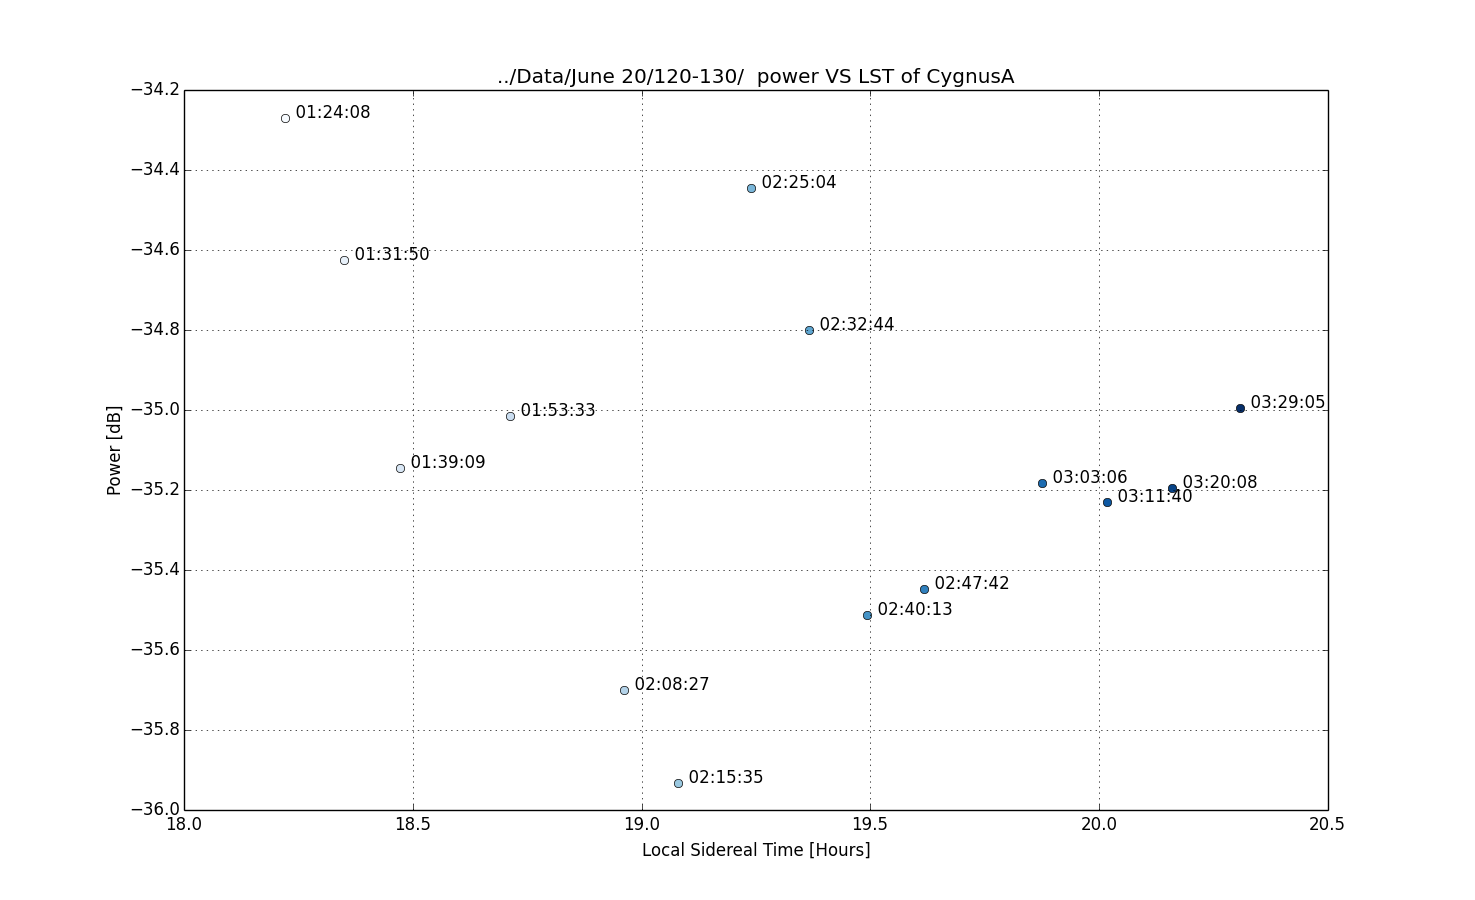
\includegraphics[width =0.85\textwidth]{spectra_plots/126127LSTdB}
	\caption{126-127 LST
\label{Fig:126127LST} }
	\end{center}
\end{figure}


\begin{figure}[H]
	\begin{center}
	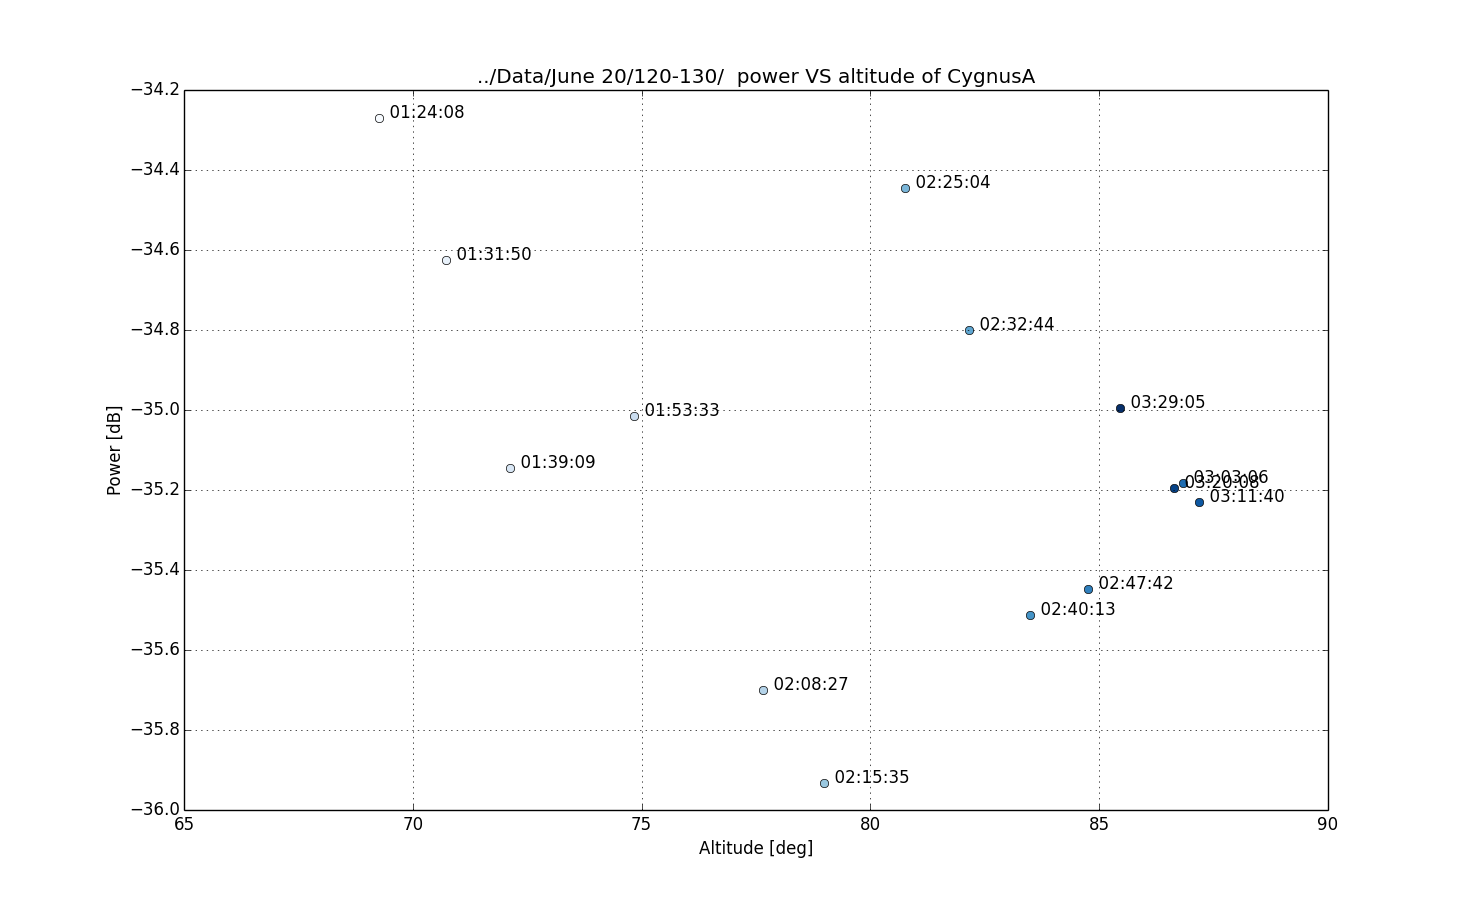
\includegraphics[width =0.85\textwidth]{spectra_plots/126127altdB}
	\caption{afga
\label{Fig:126127alt} }
	\end{center}
\end{figure}

\begin{figure}[H]
	\begin{center}
	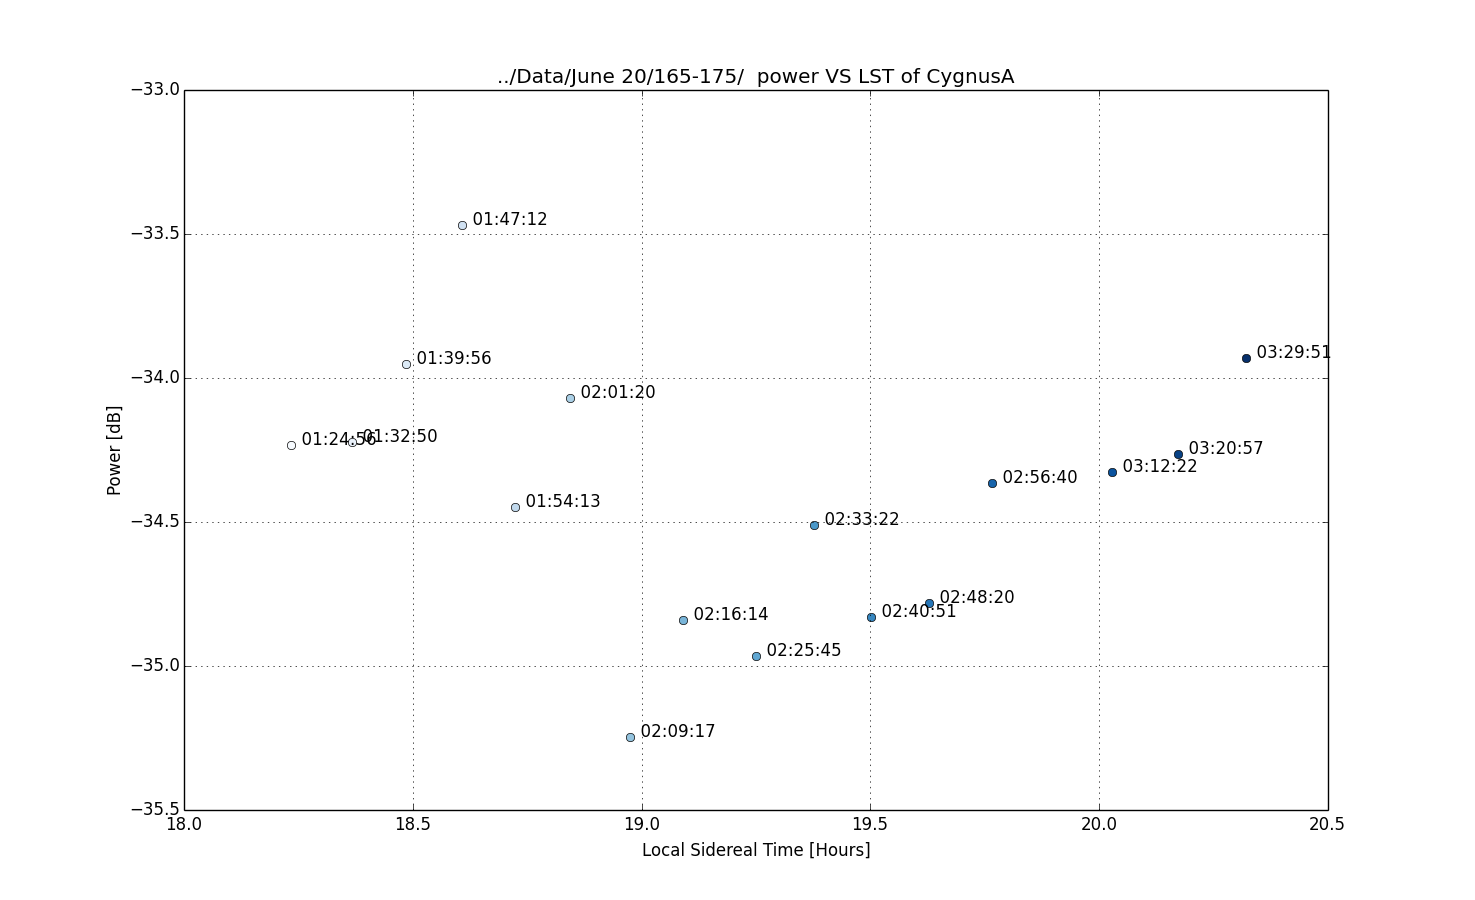
\includegraphics[width =0.85\textwidth]{spectra_plots/171173LSTdB}
	\caption{171-173 LST
\label{Fig:171173LST} }
	\end{center}
\end{figure}


\begin{figure}[H]
	\begin{center}
	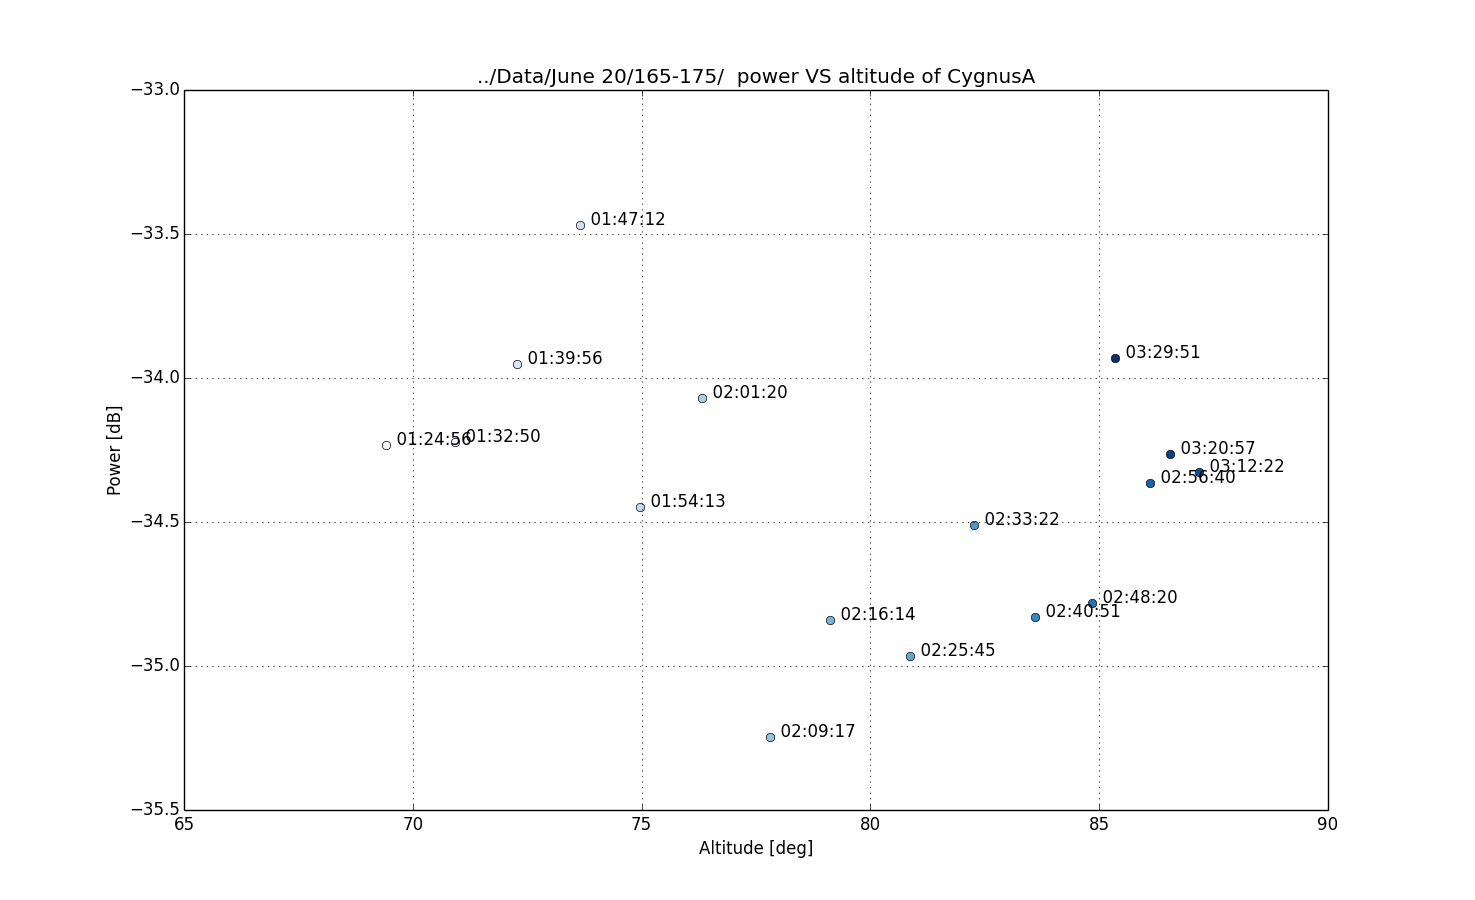
\includegraphics[width =0.85\textwidth]{spectra_plots/171173altdB}
	\caption{171-173 alt
\label{Fig:171173alt} }
	\end{center}
\end{figure}
\clearpage

\subsection{How well did we place everything}
stringent parameters affect the overall parabolic dish, surface error, geometry of rays, 
important that the hub is centered at the vertex within couple inches....

Resurvery the center for hub after telephone poles were stabilized in the ground. The telephone poles have varying diamater and along the length. 

The surrounding posts are not equidistant to the center of the hub; within ~5' between maximum post to center distance and minimum post to center distance.

The survey points in the table is defined as:
Pole 1 = the very first pivot pole, hand drilled hole; 
Pole 2 = The highest pole near the fence; 
Pole 3 = the pole closes to the shed, near where our cars are parked


\begin{table}[!h]
\centering
\begin{tabular}{|c|c|c|} \hline

Point 1 & Point 2 & Distance \\ \hline
Pole 1 & Pole 2 & 48'$\frac{1}{4}$'' \\ \hline
Pole 1 & Center & 332'' \\ \hline
Pole 1 & Pole 3 & 47'$\frac{2}{3}$'' \\ \hline

\end{tabular}
\caption{The table lists the distances between poles and center before drilling the 2 holes after locating 
the point of same horion using a theodolite and 2X4s \label{Tab:survey_dist_b4_2holes}.}
\end{table}



We measured the pole to pole distance after the center is finalized at the same height on all poles.

\begin{table}[!h]
\centering
\begin{tabular}{|c|c|c|} \hline

Point 1 & Point 2 & Distance [Feet] \\ \hline
Pole 1 & Pole 2 & 47.1 \\ \hline
Pole 2 & Pole 3 & 47.4 \\ \hline
Pole 1 & Pole 3 & 46.9 \\ \hline


\end{tabular}
\caption{The table lists the distances between poles after we finalized the center. \label{Tab:dist_p2p}}
\end{table}


ideal parabola: 
simulated parabola:
real life parabola:


 

\begin{itemize}
\item delay spectrum for configurations
\item cost
\item photos of constructed element
\item XXX hook up receiver and to a sky test ----- what is XXX?
\item measured parabolicity ---- Total station?
\item why were we right in the antenuation per reflection?
\item does the cone help?
\item how well did we place everything?
\item ways to ensure spec in field
\item mention extender as unnecessary in flat deployments
\end{itemize}

\section{Conclusion}
\label{sec:conclusion}

\begin{itemize}
\item relevance to HERA, project cost
\item link Pober et al. (2014) sensitivity/science
\item polarization matching
\item frequency coverage, need for a feed re-design.
\end{itemize}

\section{Acknowledgment}

We would like to thank SKA-SA for the site infrastructure, maintenance, and observing support
that has made this work possible, as well as the significant efforts of the staff at
NRAO's Green Bank and Charlottesville sites.  AP would like to thank M. McQuinn and A. Lidz
for helpful discussions and ionization models.
The PAPER project is supported
by the National Science Foundation (awards 0804508,
1129258, and 1125558), and a generous grant
from the Mt. Cuba Astronomical Association.

% ---------------------------------------------------------------------
% ---------------------------------------------------------------------
% ---------------------------------------------------------------------

\bibliographystyle{apj}
\bibliography{biblio}

\end{document}

\begin{figure}[H]
	\begin{center}
	\includegraphics[width =\textwidth]{}
	\caption{
\label{Fig:} }
	\end{center}
\end{figure}
